\chapter{Single-Cell EPigenome-based Inference of Activity}\thumbforchapter
\chapterauthor{Rebecca R. Snabel*, Maarten van der Sande*, Gert Jan Veenstra, Simon J. van Heeringen}
\newpage

\section{Abstract}

Single-cell RNA-seq (scRNA-seq) has proven to be a powerful tool for understanding gene expression profiles and cellular heterogeneity. However, as the quality of inferred gene regulatory network (GRN) from transcriptomic data is low, the need for more layers of information is required. Chromatin context, such as DNA accessibility and chemical modifications like H3K27ac, which are often enriched at cis-regulatory regions, improves GRN inference. Here we present SCEPIA, a computational tool that integrates scRNA-seq with a reference collection of (bulk) H3K27ac. We show that transcriptomic samples can be reliably and automatically matched to genomic samples. Moreover, by matching scRNA-seq with H3K27ac we improve the inferred transcription factor motif activities. Finally, we demonstrate the usefulness of SCEPIA on \textbf{HHCA TODO}. SCEPIA is available at \url{https://github.com/vanheeringen-lab/scepia.}

\section{Introduction}

The state of a cell's gene activity is shaped by a complex network of interacting genes, with a special role reserved for transcription factors (TFs). TFs bind to cis-regulatory DNA and change its chromatin state or interact with other transcription factors in proximity\cite{Spitz2012}. This in turn regulates the rate of transcription of the related genes. As such, to understand transcription regulation it is crucial to have an understanding of the interplay between cis-regulatory regions and transcription factors. To this end, genomic assays such as histone- and transcription factor ChIP-seq\cite{Robertson_2007}, DNAse-seq\cite{Boyle_2008}, and ATAC-seq\cite{Buenrostro_2013} have been developed. These assays allow for the precise measurement of histone modifications, transcription factor binding, and DNA accessibility, and consequently for the inference of cis-regulatory elements and their related TFs.

Single-cell transcriptomics has emerged as a rapidly expanding field, allowing researchers to explore the gene expression profiles of diverse cell types with increasing ease and affordability. However, when it comes to examining DNA accessibility, transcription factor binding, and histone context, crucial aspects of transcription regulation, challenges persist. Single-cell ATAC-seq (scATAC)\cite{Buenrostro2015_sc}, while immensely valuable, remains costly and generates sparser data compared to single-cell transcriptomics and bulk genomic methods\cite{Li2021}. Similarly, single-cell CUT\&Tag (scCUT\&Tag)\cite{Bartosovic2021}, a method able to measure histone modifications as well as transcription factor occupancy on a single-cell level, \textbf{something about difficult and expensive}. Consequently, many laboratories encounter difficulties in adopting these techniques.

As genomic information is crucial for understanding gene regulation, but remains hard to acquire in single-cell data, linking single-cell transcriptomic data to bulk reference genomic databases is a standard practice. For instance, the computational tool SCENIC infers transcription factor co-expression regulons based on single-cell transcriptomic data, and refines these regulons based on the presence of relevant motifs in cis-regulatory regions surrounding the genes within a reference genomic database\cite{Aibar_2017,VandeSande2020}. Similarly, the computational tool SCRIP combines single-cell ATAC-seq with a reference database to get a blended bulk and single-cell per-gene signal. This approach mitigates the downsides of single-cell ATAC-seq, which is noisy and sparse, but still profits from its resolution\cite{Dong2022}. These tools show a successful integration of single-cell data with a reference database. And given that the information in genomic assays and transcriptomic assays is partially redundant\cite{Wang2016,GonzlezRamrez2021}, the opportunity arises for automatically associating transcriptomic data with genomic assays of a similar cell type. Furthermore, the combination of both genomic and transcriptomic data has been shown to enhance the inference of gene regulatory networks\cite{Xu_2020,Kamal_2021}. This poses an intriguing concept: automatically linking single-cell transcriptomic data to a bulk genomic reference, which in turn potentially improves transcription factor motif activity inference.

Here we explore the question of whether (single-cell) transcriptomic data can be linked to a genomic reference collection to improve transcription factor motif activity inference. This approach has two advantages. First, single-cell RNA-seq is cheaper and easier to perform than single-cell genomic assays (scATAC, scCut and Tag). Moreover, by automatically linking single-cells to a genomic reference one gets multiome data. Second, by using the reference data for motif activity inference it is possible to compare gene expression and motif acvitiy, and remove spurious interactions. We call this approach Single-cell EPigenome-based Inference of Activity (SCEPIA). We test on HHCA..

% This reference database can be used for motif scanning.  To \textit{test} how SCEPIA performs on real data, we have used the latest version of the human Heart Cell Atlas v2 (REF XXX HHCA v1, HHCA v2). The version 2 of this dataset additionally consists of single-cell chromatin accessibility data alongside transcriptomic data from the same nuclei, by combining both versions of the atlas the authors produced an extensive atlas covering the different tissues and cellular subtypes present in the human adult heart. A lot is known about different cellular markers and regulators of the different cell types within the heart, however, much can also still be gained from more detailed research on further epigenetic regulation within the heart, and the transcriptional actors contributing to this. However, in this research only the openness of the chromatin is captured, not the more detailed information on the histone modification differences, which can inform on whether an accessible region acts as an active enhancer. Cardio-vascular diseases are still the number one cause of deaths worldwide (\href{https://doi.org/10.1161/CIR.0000000000001123}{https://doi.org/10.1161/CIR.0000000000001123}), and the ability to research intricate differences between healthy and diseased tissues in a multimodal setting, will help to gain more understanding of the complex (dis)regulation happening in these tissues, also on the less researched field of epigenetic on a cellular//cell type level. 

% The availability of the single-cell chromatin accessibility data, can be used as an epigentic read-out and thereby brings us one step closer to the type of data SCEPIA will infer. This allows us to validate the performance of our tool in predicting epigenetic/transcriptional regulation from a single-cell transcriptomic dataset. // SCEPIA infers per single cell the active enhancer signal from public ChIP-seq data resources, although accessibility of the chromatin is one read-out of the effect of such active enhancer signal.

\section{Results}

\subsection{Matching Regulatory Potential and Transcripts Per Million}

We hypothesized that incorporating a measure of cis-regulatory element activity, such as ATAC-seq or H3K27ac ChIP-seq, would be beneficial to identify transcription factor motif activity from single-cell transcriptomic data, even when this is not experimentally measured. Here, we used the \textit{regulatory potential} to match single-cell RNA-seq profiles to a collection of known H3K27ac ChIP-seq profiles. The regulatory potential is defined as the weighted average H3K27ac signal per gene \cite{Wang2016}. To determine how well regulatory potential specifically matches RNA-seq data for identical (or similar) cell types, we obtained data from 96 human RNA-seq cell types and 121 human H3K27ac cell types from ENCODE\cite{encode_dcc} (Supplementary \textbf{Table SX}). We calculated the regulatory potential for all H3K27ac samples (see Methods). We then computed the correlation coefficient for all possible combinations of regulatory potential and RNA-seq values (Fig. \ref{fig:bulk_comparison}). In general, the regulatory potential shows only a high positive correlation for a subset of the transcriptomic data, indicating that the measure captures a cell type-specific signal. The mean correlation coefficient for identical cell types between regulatory potential and transcripts per million (TPM) was found to be 0.53 with a standard deviation of 0.14. In 64\% of instances, the regulatory potential of a given cell type exhibited the highest correlation with the TPM of the same cell type. Furthermore, in 77\% of the cases, the highest correlation was observed with a tissue sharing the same ontology term. As noted previously \cite{Wang2016}, the specific parameters used for calculating regulatory potential do not significantly impact the results. For this specific analysis, the H3K27ac signal in the promoter region alone is sufficient to predict the TPM (table \ref{table:correlations}). In summary, our findings suggest that a collection of H3K27ac regulatory potential can effectively serve as a reliable classifier for characterizing cell states based on transcriptomic data.

\begin{figure}
    \centering
    \includegraphics[width=1\linewidth]{ch.scepia/imgs/celltypes.png}
    \caption{\textbf{Transcriptomic counts are a reliable predictor for H3K72ac cell state and automatically matching assays improves motif activity inference.} \textbf{(A)}: The Pearson correlation coefficients between all combinations of 121 H3K27ac regulatory potentials and 96 RNA TPMs. In 77\% of the comparisons, the highest correlation between TPM and regulatory potential was observed between samples with the same ontology term. \textbf{(B)}: Motif activities based on samples automatically matched to a reference H3K27ac collection are more accurate than on transcriptomic data alone. The motif activities between 5 random cell types are inferred based on their H3K27ac signal in their top 25,000 differential enhancers (100 permutations). The naive approach to motif activity inference with only transcriptomic data is to assume that the TPMs of transcription factors are directly related to their motif activity. The naively inferred motif scores only have an average correlation score of 0.04 with the true motif scores. The regulatory potential-based approach automatically matches a transcriptomic sample to an H3K27ac sample and infers the motif activity scores on their top 10,000 differential enhancers (\textbf{mean of XX}). The identical sample in the H3K27ac reference database \textbf{is held out}. Finally, as the motif activities are based on the top 25,000 differential enhancers, the subset models the correlations between motif activities on the top 10,000 and top 25,000 differential enhancers (\textbf{mean of XX}).}
    \label{fig:bulk_comparison}
\end{figure}

In general, the H3K27ac signal in regulatory sequences can be used to determine motif or transcription factor activity\cite{FANTOM2009,Balwierz2014,Madsen_2017}. This motif activity, which quantifies the contribution of each motif to H3K27ac peak strength, has been shown to be a powerful measure of the relevance of a transcription factor for a specific cell state. The relationship between RNA-seq and regulatory potential led us to assume that transcription factor motif activity can be inferred from transcriptomic data, through an intermediate collection of matched H3K27ac data. As the reference collection contains a limited number of cell types, an exact matching cell type may not always be available for a specific cell type measured by RNA-seq. Therefore, we decided to calculate a composite measure of motif activity, based on a combination of reference cell types. To calculate this measure, we regressed the TPM values of the 2,000 most variable genes of a collection of cell types against our regulatory potential database. From there, we selected the top 50 cell types based on the absolute regression coefficients and identified the top 10,000 most differentially enriched cis-regulatory regions within these 50 cell types. Subsequently, we calculated the motif activity using these enhancers, and obtained the final motif scores by taking the dot product of motif scores and regression coefficients. 

To test our composite activity score, we made one hundred random subsets of five tissues common to both our H3K27ac reference database and transcriptomic dataset. Our first step involved establishing a ground truth for motif activities by conducting a motif scan on the top 25,000 most differentially enriched enhancers within each of these five tissues. Here, enhancers were defined as peaks within the REMAP dataset located more than 2kb away from the transcription start site. A naive approach to estimating motif activity based solely on transcriptomic data would assume a direct one-to-one translation between the transcripts per million (TPM) values of a transcription factor and its motif score. However, as Figure \ref{fig:bulk_comparison}B illustrates, this naive approach displays a particularly poor correlation with our ground truth data. Instead, our approach based on regulatory potential demonstrates a significantly improved correlation compared to the naive method (Figure \ref{fig:bulk_comparison}B). Note that the cell types used for the ground truth are excluded from the reference database. Finally, to assess the sensitivity of our approach to the choice of enhancer set, we compared the ground truth data based on the top 25,000 most variable enhancers with that based on the top 10,000 most variable enhancers. Taken together, these analyses show that RNA-seq can be reliably matched to H3K27ac in a cell type-specific manner and that this data can be used to estimate transcription factor activity. See supplemental \textbf{figure XXX, still to come} for parameter sweep, that shows ??. 

\subsection{Single-Cell EPigenome-based Inference of Activity}

The previous section demonstrates the reliable matching of gene counts to an H3K27ac reference using regulatory potential. This matching process enhances the inference of transcription factor motif activity, even in the case where the exact matching cell type is absent in the reference. Given the ability of single-cell sequencing to finely separate between cell types, this methodology can be effectively extended to single-cell RNA-seq. Additionally, the increased number of measurements in single-cell sequencing facilitates more sophisticated significance testing, further strengthening the analytical capabilities of the method (\textbf{this is a bit sketchy though..}).

\begin{figure}
    \centering
    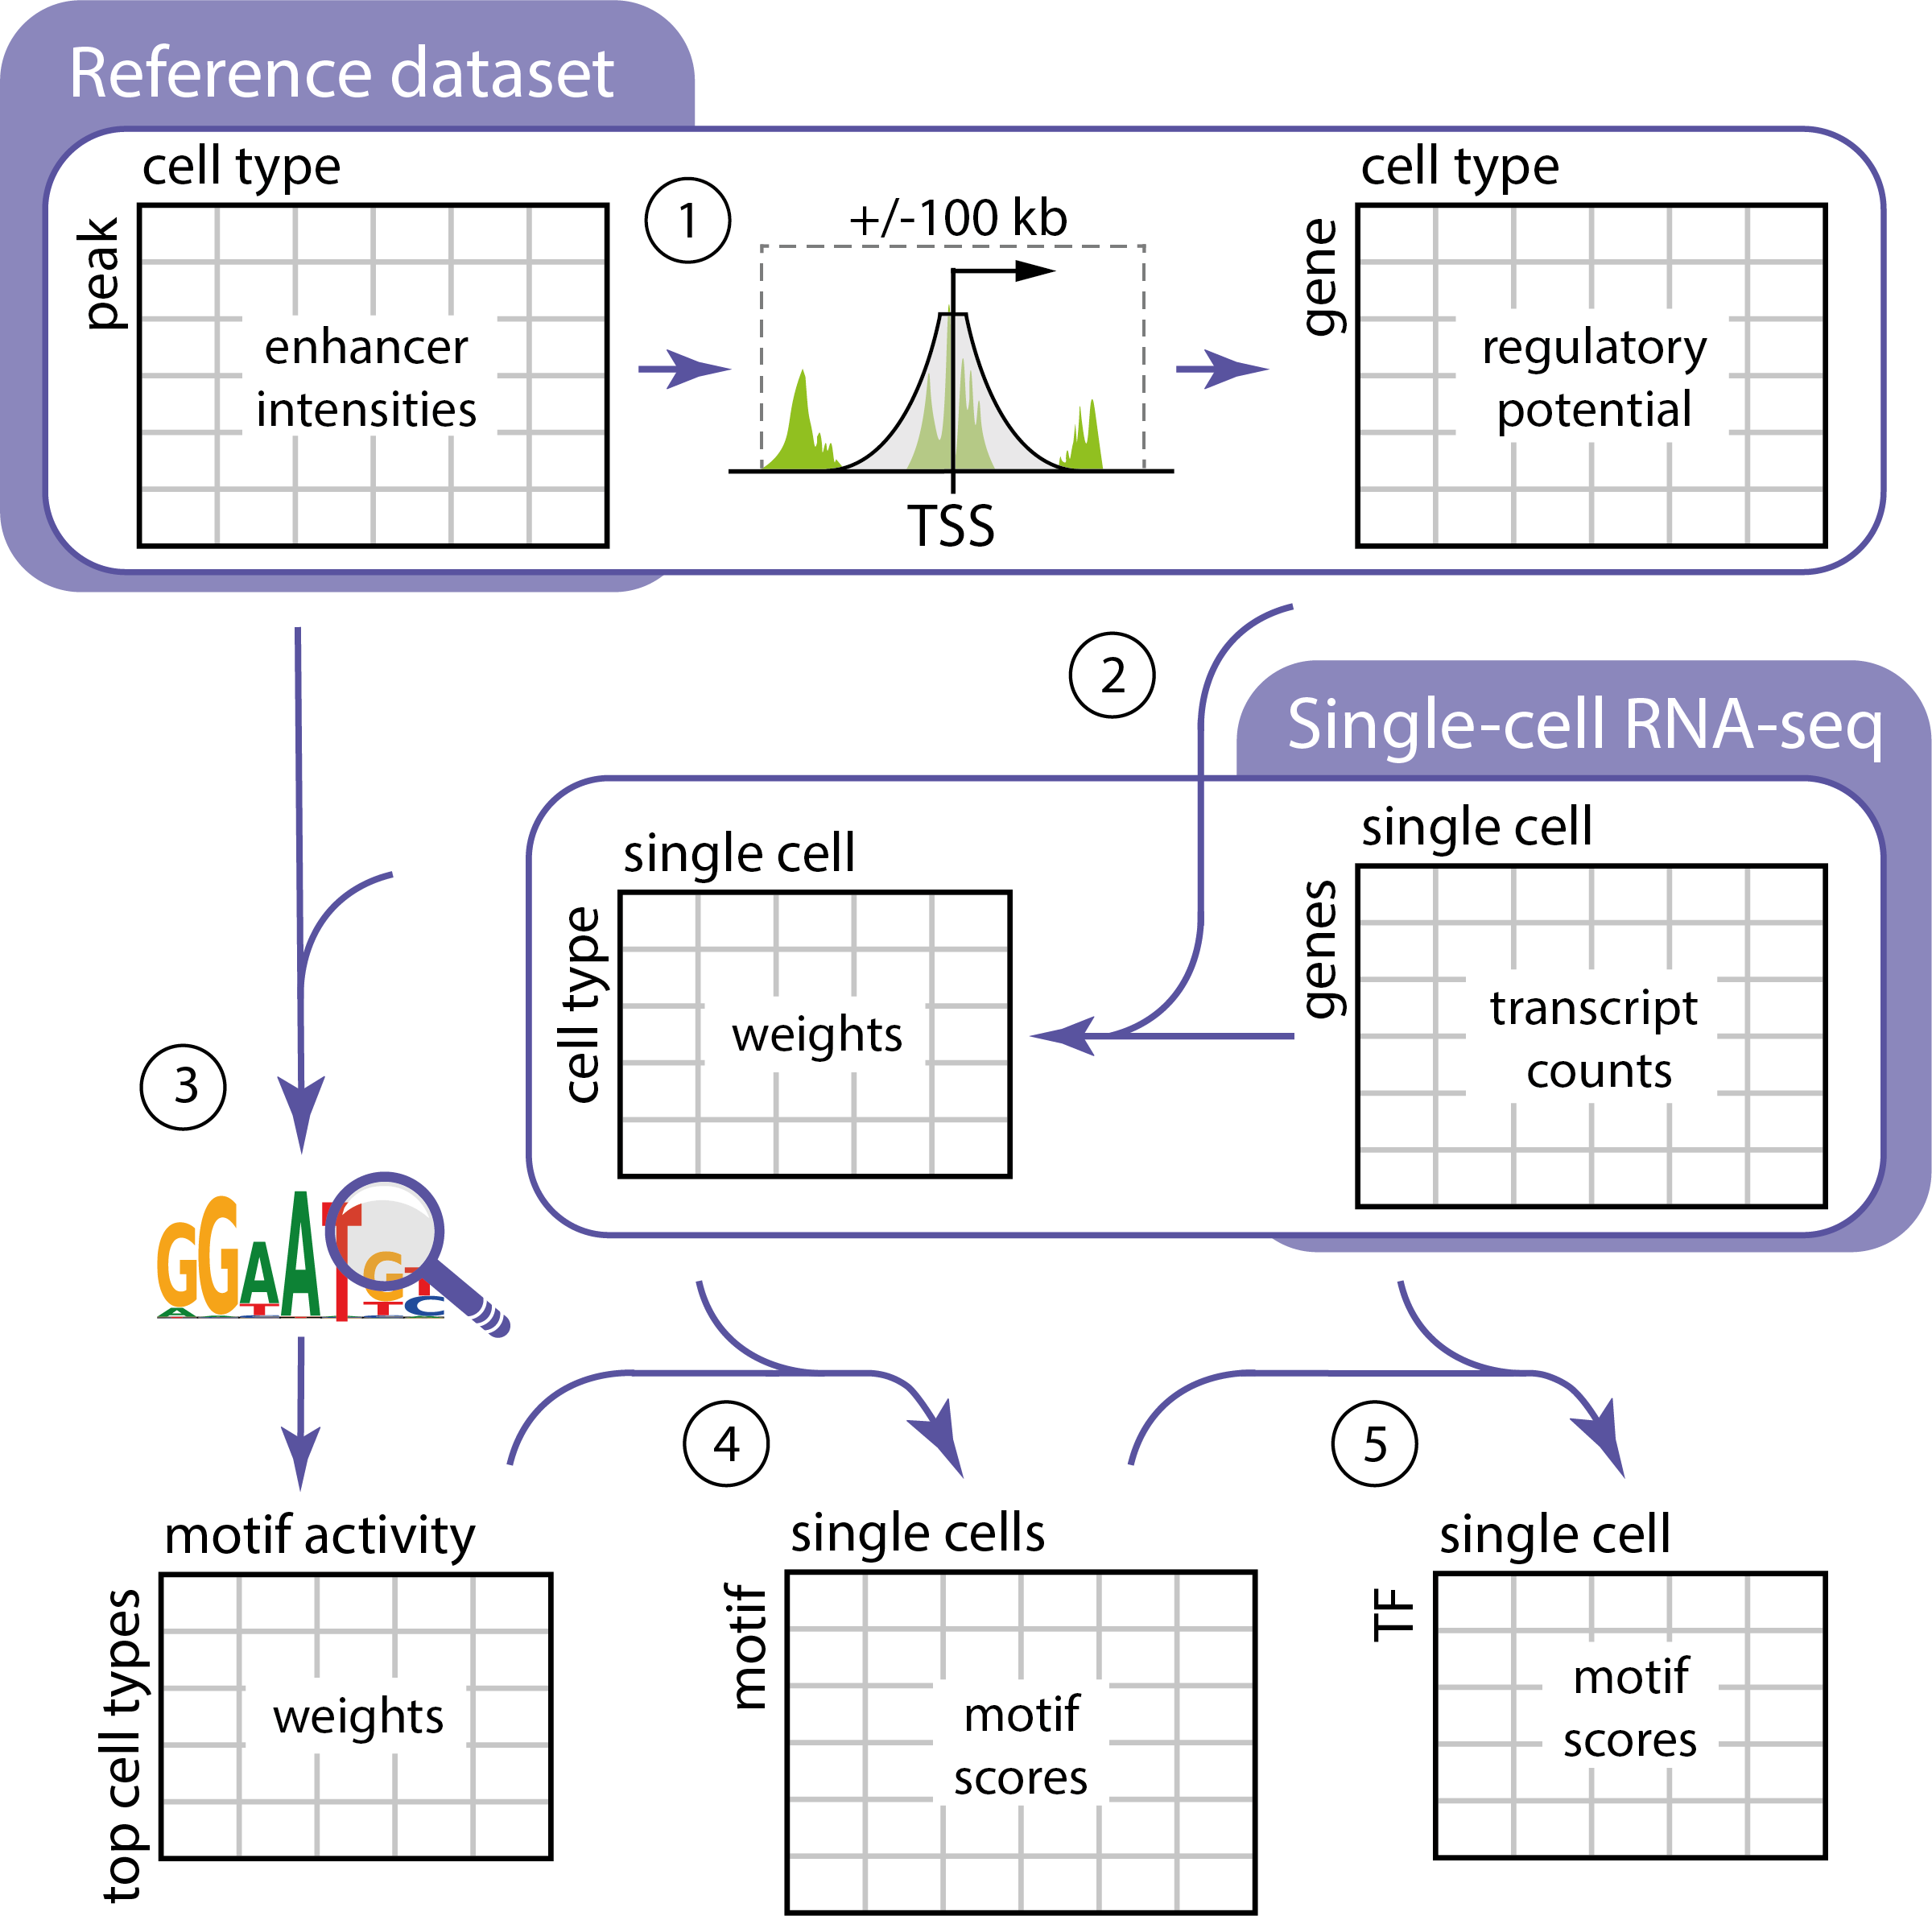
\includegraphics[width=1\linewidth]{ch.scepia/imgs/20231106_OverviewFigure_SvH_v2.png}
    \caption{\textbf{Schematic overview of Single-Cell EPigenome-based Inference of  Activity (SCEPIA).} See the methods for an extensive explanation per step. \newline 
    \textbf{Step 1}: Calculate the regulatory potential from distance-weighted chromatin-assay intensities around each gene for each cell type in the reference collection.
    \textbf{Step 2}: Regress the single-cell gene expression on the regulatory potential. Keep the top 50 cell types with the absolute highest regression coefficients, and use those as the cell type weights for each cell.
    \textbf{Step 3}: Select the top 10,000 most differential \textbf{peaks/enhancers/...} between the top 50 cell types, and use them for motif activity inference.
    \textbf{Step 4}: Take the dot product between the motif activities and the cell type weights, resulting in motif activities for each motif per cell. Motif activities are scaled to a motif score between 0-1. 
    \textbf{Step 5}: Calculate the correlation coefficient between all pairs of TF gene expression and motif activities. A permutation test between gene expression and motif activities allows for the estimation of the statistical significance of their relation.}
    \label{fig:scepia_overview}
\end{figure}

To test SCEPIA on a scRNA-seq data source for which matching single-cell chromatin accessibility data was available, we used the human Heart Cell Atlas v2 (hHCA) multiome data (\cite{Kanemaru2023}). Since SCEPIA performs motif activity inference solely informed on the scRNA-seq data, we evaluate how this compares to motif activities found in the actual accessible chromatin of these cells. Furthermore, SCEPIA selects regulatory factors based on motif activity combined with the TF's expression levels and we validate how this compares to a selection based on motif activity alone. // we validate if SCEPIA's selection of regulatory factors based on expression of the TF as well as its predicted binding motif activity, improves the selection based on motif activity alone.

To confirm that matching cell types \textcolor{red}{on inferred transcriptomes} also works for a single-cell source, we compared the inferred annotation by SCEPIA with the cluster annotation as profided by the authors. // First, we ran SCEPIA on the whole hHCA scRNA-seq dataset and compared the inferred annotation with the cluster annotation as provided by the authors. SCEPIA correctly assigned the atrial and ventricular cardiomyocyte clusters correctly to heart ventricle and cardiac atrium, respectively. The fibroblasts, neural cells and mural cells (i.e. smooth muscle cells or pericytes of the vasculature), all matched to tissue or cell types similar to their identity, albeit these originated from a different organ or tissue (i.e. lung or tibia) (Figure 3A). Also the myeloid and lymphoid clusters were matched with a cell type of the correct major immune lineage branch, namely CD14+ monocytes and CD8+ T cells, respectively. It was more difficult for SCEPIA to correctly match the endothelial cells, which showed the best match with heart left ventricle and only to a lesser degree to an endothelial cell type (Fig. \ref{fig:scepia_annotation1})\textcolor{red}{, however, the endothelial cells make up a large fraction of the heart's myocard, as can also be deduced from the cluster size within the atlas, which could explain this result. Ultimately in SCEPIA's analysis, the endothelial cluster was represented by a combined signature of left ventricle and an endothelial cell type. Likewise, the adipocytes are represented by a mixed signature of right cardiac atrium and adipose tissue (Fig \ref{fig:scepia_annotation1}).} For the mesothelial cluster, there was no matching cell or tissue type available in the ENCODE database, which could explain the lack of any strong matches for this cluster. These results highlight that SCEPIA matched the majority of the clusters to similar cell types in the ENCODE reference. 

\textcolor{red}{After the initial step of matching the single cells to the cell types of the H3K27Ac reference, we now want to determine which transcriptional regulators SCEPIA considers to be of importance in these cell clusters.} Within the top hits identified by SCEPIA, multiple known markers for cell types present in the atlas were observed (Figure 3B). \textit{FLI1}, \textit{ETS1} and \textit{KLF2} are known for their roles in immune and endothelial cells (REF XX). Other examples include the well-known cardiomyocyte regulators such as \textit{TBX5} and \textit{HEY1}, \textit{PPARG }as a regulator for adipocyte differentiation, \textit{SOX17} marked specifically the endothelial cells and RUNX1 as lymphoid marker (Figure 1C). The \textit{TBX5} predicted motif activity in the cardiomyocyte clusters follows the patterns of expression, with further increased levels in the atrial cluster specifically. The motifs identified for \textit{SOX17} and \textit{RUNX1} showed variable accessibility across and within various clusters of the atlas, although both were further enriched in the endothelial and lymphoid cluster respectively (Figure 1C). \textit{BACH2} is a known repressor and immune-regulating transcription factor and implicated in neural differentiation (\href{https://www.ncbi.nlm.nih.gov/pmc/articles/PMC8934237/}{https://www.ncbi.nlm.nih.gov/pmc/articles/PMC8934237/}, \href{https://pubmed.ncbi.nlm.nih.gov/16631738/}{https://pubmed.ncbi.nlm.nih.gov/16631738/}), and IKZF1 is described as both repressor and activator in immune cells (\href{https://www.ncbi.nlm.nih.gov/pmc/articles/PMC5865415/}{https://www.ncbi.nlm.nih.gov/pmc/articles/PMC5865415/}). The latter two were identified by SCEPIA as repressors, deduced from the anti-correlation between their mRNA levels and predicted motif activities. \textcolor{red}{BACH2 expression was highest in the neural and lymphoid cluster, whereas the predicted motif (bZIP.0003) activity in both of these clusters was decreased, compared to other clusters (myeloid and endothelial showed highest motif activity; Figure S4XX). This is indicative of a repressor function in the neural and lymphoid clusters, however, for the other clusters this indicated an activating role. BACH2 is a known repressor for myeloid lineages and in neural differentiation, however in some cases the factor is described as an activator (REFXX), this proved a difficult mechanism of regulation for SCEPIA to infer solely from the transcriptome data and reference. This could be explained by a lack of certain cell types in the H3K27Ac reference, which would be able to better capture the intricate regulation occurring in myeloid cell populations (REF XX; \href{https://www.nature.com/articles/ni.3024}{https://www.nature.com/articles/ni.3024}).}
\begin{figure}
    \centering
    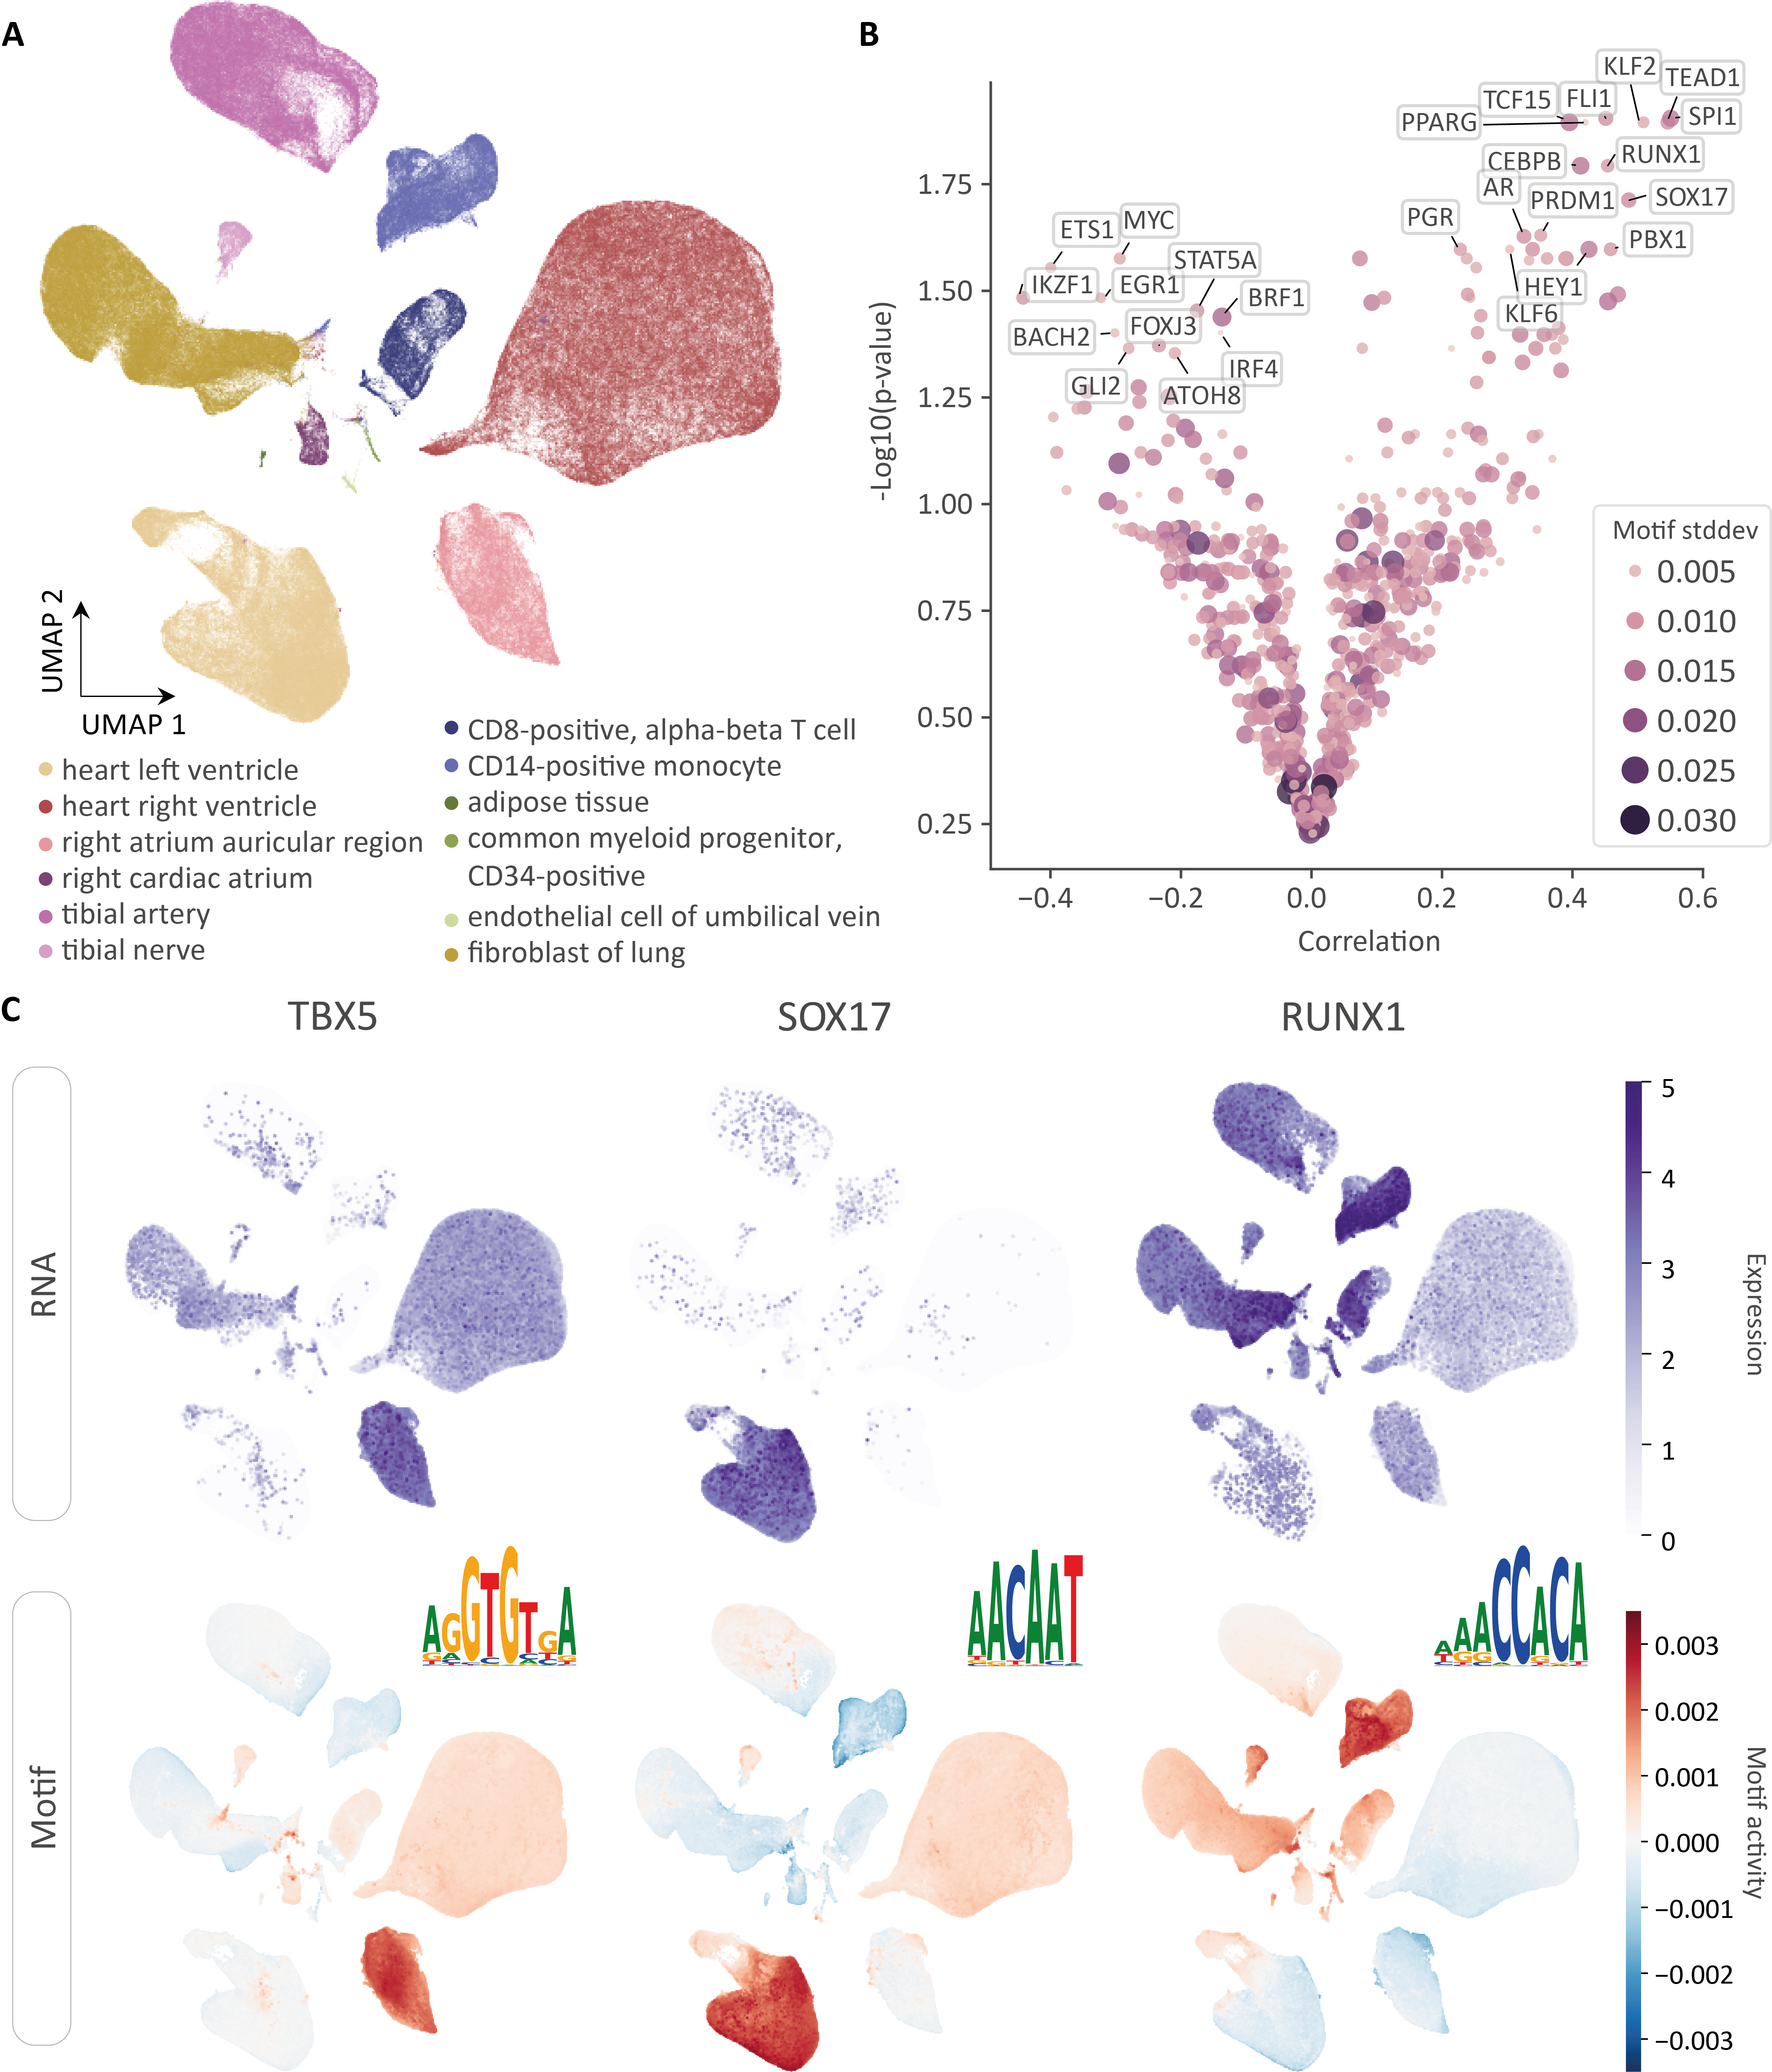
\includegraphics[width=0.75\linewidth]{ch.scepia/imgs/SCEPIA_allCells_Fig1_v9.png}
    \caption{\textbf{SCEPIA run on the Human Heart Cell Atlas} (a) UMAP representation, based on UMAP coordinates provided by the original study\cite{Kanemaru2023}, with cluster annotation labels as predicted by SCEPIA. (b) Volcano plot of SCEPIA hits, labels of the top 15 of both correlating as anti-correlating hits are indicated, based on p-adj < 0.05 values. Dot size and color labels are based on the motif score standard deviations.  (c) Expression levels (top) of 3 well-known markers, TBX5 (cardiomyocytes), SOX17 (endothelial cells), RUNX1 (blood cells), and their predicted motif [[scores/activity]] by SCEPIA (bottom), printed on the UMAP as shown in (a). Sequence logos of the binding motifs are indicated, with the GimmeMotifs database identifiers (left to right): GM.5.0.T-box.0005, GM.5.0.Sox.0021, GM.5.0.Runt.0003. }
    \label{fig:scepia_hhca1}
\end{figure}

\textbf{Benchmark SCEPIA on Single-Cell Data}

Next, we set out to more broadly assess SCEPIA's results, as well as its reproducibility. To this end, we split up the hHCA scRNA-seq data into seven random subsets of 100K cells each. Simultaneously, we ran GimmeMotifs Maelstrom motif analysis on the pseudobulk of the scATAC-seq clusters (from now on referred to as maelstrom analysis), to explore cell-type specific motif activities in the measured accessible regions. SCEPIA is designed to infer enhancer activity and this motif analysis on pseudobulk scATAC-seq therefore functions as the closest approximation to a \textit{ground truth} for this experiment. We correlated the motif activities computed from the maelstrom analysis with the expression levels of each of their TF binders per cell type, and for each subset. This comparison is done without any prioritization between motifs and TFs, other than taken into account the information on predicted motif-binding factor links, and we therefore refer to this as the naive comparison. The naive comparison resulted in coefficients ranging from r = -0.03 to 0.27 (Fig. \ref{fig:sc_benchmark} blue) \textcolor{red}{and represents the degree of similarity between motif activities and the expression levels of its binding TFs, taken from the best matching multimodal data source.}

To benchmark SCEPIA against these results, the analysis on each of the seven subsets were compared to the maelstrom analysis. The significant hits (p-adj < 0.05) were selected and their inferred motif activities averaged per cell type. These averages were correlated to the computed activities for the same motifs from the maelstrom analysis. Interestingly, the mean coefficients per cell type in these correlations, were consistently higher (up to r = 0.6 for the myeloid cluster) than found with the naive comparison, except for the mesothelial cell cluster (Fig. \ref{fig:sc_benchmark} orange). However, these scores differed substantially across the different cell types.

Since some of the cell types appeared to score worse (cardiomyocyte clusters, fibroblastst and endothelial cells, averaged r < 0.4), than others (immune cell cluster, averaged r > 0.4), we added a step to achieve better representation of each cell type in the data. This was done by adding a step of geometric sketching (geosketch) in the pre-processing of the data (REF XX \& \href{https://www.cell.com/cell-systems/fulltext/S2405-4712(19)30152-8}{https://www.cell.com/cell-systems/fulltext/S2405-4712(19)30152-8}) (see Methods), and before SCEPIA was run on each of the seven subsets. This improved the correlation coefficients with the maelstrom results of most cell types - even the immune cell clusters, but especially of the cardiomyocyte, fibroblast and endothelial clusters (Fig. \ref{fig:sc_benchmark} green). The neural and adipocyte, mural and mesothelial cell-clusters achieved more variability in their coefficients, obtained equal or worse coefficients after addition of the geosketching, respectively. \textcolor{red}{Although the geometric sketch was not able to alleviate SCEPIA's issues with some cell types,} adding this step to pre-processing did improve the tool's performance for the majority of the cell clusters. 
\begin{figure}
    \centering
    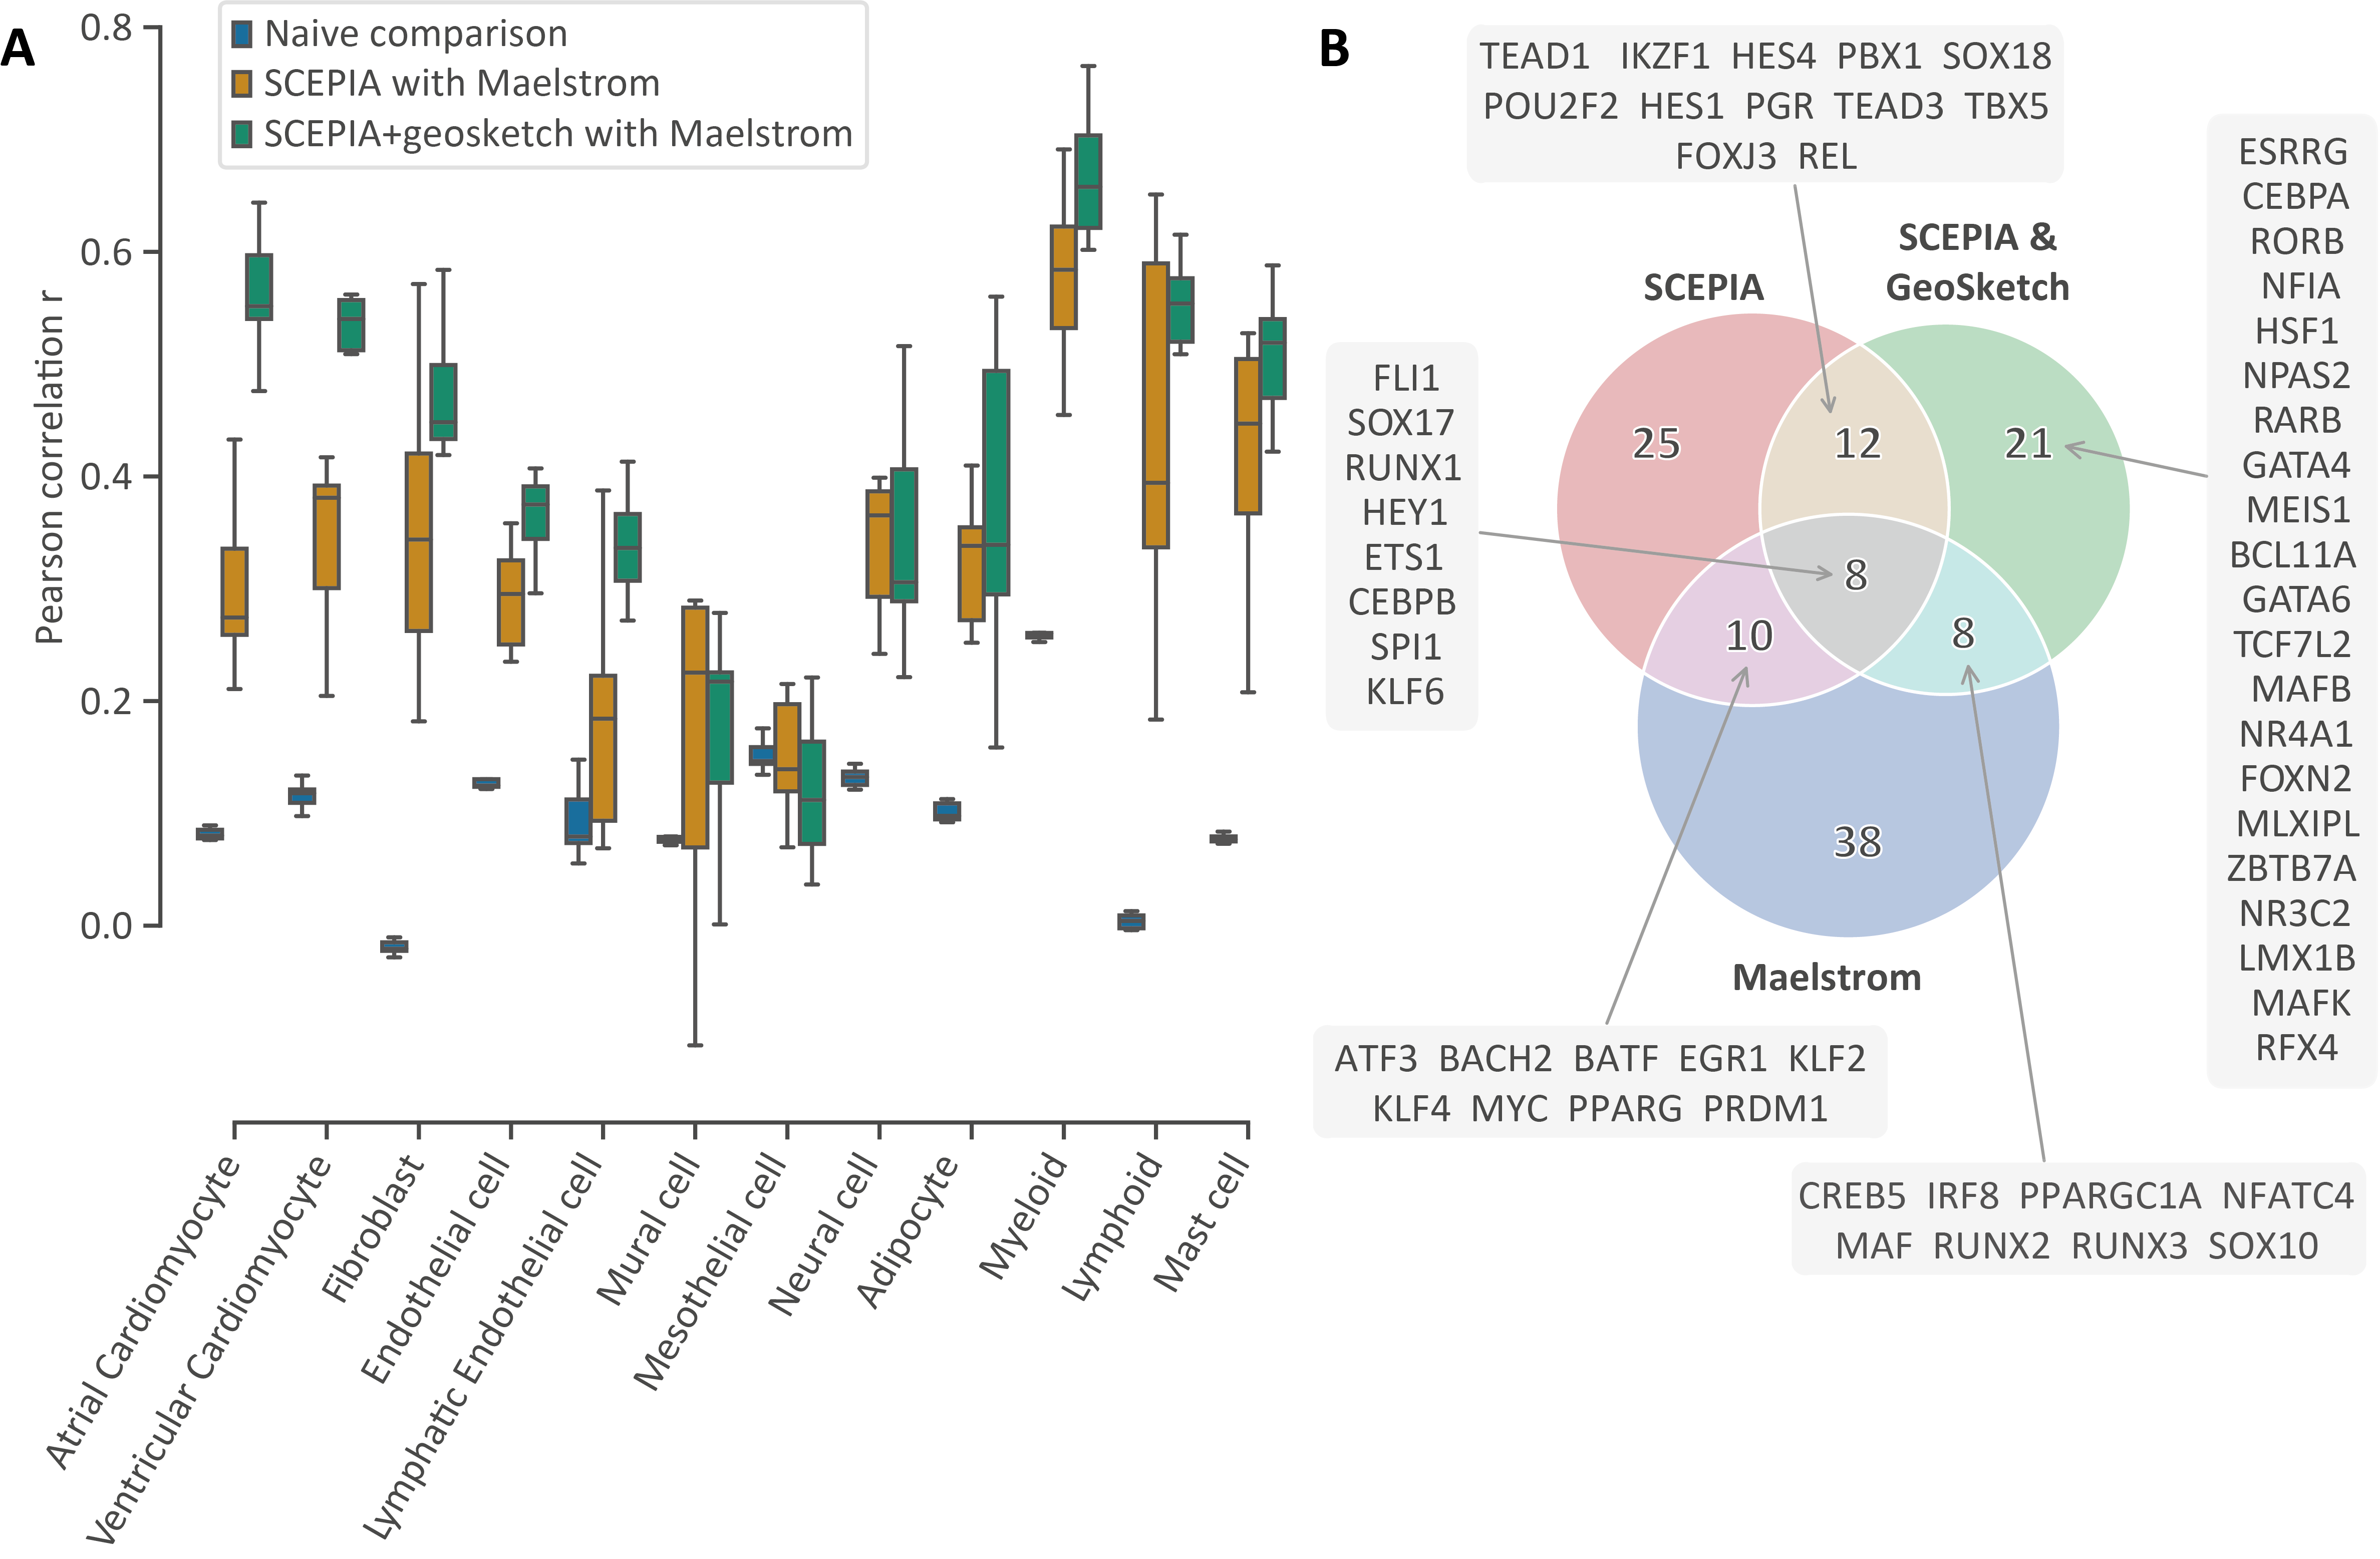
\includegraphics[width=0.75\linewidth]{ch.scepia/imgs/Fig_OverlappingHitsBetweenSCEPIAGEOANDMAELSTROM_v7.png}
    \caption{SCEPIA sc benchmark vs Naive vs Geosketch}
    \label{fig:sc_benchmark}
\end{figure}

\textcolor{red}{\textbf{Comparison of Biological Findings Across the Methods // Comparing SCEPIA with Maelstrom Motif Activities} }
Since the geosketch improved SCEPIA's performances across multiple cell types, we also reduced the full dataset to a sketch of 20K cells and reran SCEPIA (Fig. \ref{fig:geoscepia_results}). This resulted in overlapping hits with the former run of SCEPIA on the full dataset (20 hits of the 49 total hits), partial overlap with TFs linked to motif hits identified with maelstrom (16 hits; Figure 4B). Multiple overlapping hits between both SCEPIA runs on the full dataset and the maelstrom analysis, are known for their roles in cardiac cells, again FLI1 and SOX17 were present in all analyses, as well as HEY1 (cardiac progenitor marker) and ETS1 (lymphoid marker). Another example found in the first SCEPIA run and identified as a repressor, was BACH2. Maelstrom analysis also pointed to differential accessibility for a BACH2-binding motif and indicated enrichment in the fibroblast, endothelial and mesothelial cluster. SCEPIA also inferred increased motif accessibility for BACH2 in these same clusters, with additional enrichment in the myeloid and mural cells (Figure S4XX). 

However, there were also differences between the two SCEPIA runs. For instance, different GATA4 and GATA6 both known for their roles in cardiac (mesoderm) development and indicated with increased motif accessibilities in the cardiomyocyte clusters, were only identified after performing the geosketch (Figure \ref{fig:scepia_features1}A-B; \href{https://pubmed.ncbi.nlm.nih.gov/8660897/}{https://pubmed.ncbi.nlm.nih.gov/8660897/}, \href{https://www.ncbi.nlm.nih.gov/pmc/articles/PMC8916722/}{https://www.ncbi.nlm.nih.gov/pmc/articles/PMC8916722/}). In the run without geosketch, SCEPIA identified only GATA1 which showed a combination of specific expression and motif enrichment in mast cells,\textcolor{red}{ a link that can be made based on literature (\href{https://pubmed.ncbi.nlm.nih.gov/12566412/}{https://pubmed.ncbi.nlm.nih.gov/12566412/}; \href{https://ehoonline.biomedcentral.com/articles/10.1186/s40164-015-0024-z}{https://ehoonline.biomedcentral.com/articles/10.1186/s40164-015-0024-z}).} Besides this, RUNX1 was identified in both runs and in maelstrom. Specifically in the geosketch SCEPIA analysis RUNX2 and RUNX3 were added to the list, and the predicted motif for all of these factors (Runt.0003) was in the run with geosketch more restricted to immune cells, whereas in the other SCEPIA run the motif accessibility was also spread across for instance, the mural, neural and fibroblast cells (Figure \ref{fig:scepia_features1}C-D). 

Also some specific geosketch SCEPIA hits overlapped with the variable motifs as identified in the maelstrom analysis. PPARGC1A is an example of this and the exact same motif SCEPIA picked up, was identified to be variable in the maelstrom analysis (C2H2\_ZF.0037). Furthermore, the pattern of activity for this motif overlapped between the two methods, with stronger enriched in the adipocyte, fibroblast and myeloid cluster (Figure \ref{fig:scepia_features1}E, G). Motif activity of PPARGC1A is highest in adipocytes, endothelial and fibroblast cluster, as both identified with SCEPIA and Maelstrom, whereas the expression is found highest in the cardiomyocyte clusters. This is why SCEPIA identified PPARGC1A as a repressor. Another example concerns the SOX gene family. SOX17 and SOX18 were already identified in the first SCEPIA run, coupled to motifs with similar accessibilities over the clusters, additionally SOX13 was identified in that run (Figure \ref{fig:scepia_features1}F). SOX10 however, was only identified in the run pre-processed with geosketch, and was specifically expressed in the neural cluster (Figure S4XX). In the maelstrom analysis, two in the top three highest enriched motifs of the neural cluster, concerned motifs for SOX10 (Sox.0018 and Sox.007), with highest accessibility in the neural cluster, \textcolor{red}{followed by the fibroblast cluster for the one motif and by the endodermal cells in the other}. In the SCEPIA analysis the predicted motif for SOX10 (Sox.0034) showed this same level of specificity of enrichment (Figure \ref{fig:scepia_features1}H).

Differences between the maelstrom analysis and SCEPIA runs, included IKZF1, which was picked up by SCEPIA and linked to a motif with abundant accessibility and only a specific depletion of signal in the immune clusters (Fig. \ref{fig:scepia_features2}B, D). Other examples include, TBX5 and MEIS1, both well-known cardiac mesoderm markers, alongside ESRRG. Some of the binding motifs for these factors, according to the predictions, showed a level of activity across multiple clusters in the dataset, and only in combination with their expression made these factors more specific as potential transcriptional regulators (example of ESRRG, Fig. \ref{fig:scepia_features2}A, C). Conversely, there were also hits in Maelstrom, that were not identified in any of the SCEPIA runs. The MEF2 transcription factor family showed a specific motif enrichment in the accessible chromatin of the cardiomyocyte and mural cell cluster, however, the expression levels for MEF2A-D were very consistent over the different cell types in the dataset, which could explain this result (Fig. \ref{fig:scepia_features2}E).

\section{Discussion}

In this study, we present SCEPIA, a computational method for the inference of transcription factor motif activities based on transcriptomic data and a reference H3K27ac collection. We show that one can reliably match cell types based on transcriptomic abundance and H3K27ac-based regulatory potential\cite{Wang2016}, both in the case of bulk and single-cell transcriptomics. The chromatin context of the matched data can be used for motif activity inference, which in turn can be integrated with transcriptomic information. As such it is a big improvement over the case when only transcriptomic data is available. We test the inferred \textbf{regulatory} transcription factors on the human heart cell atlas, and show that XYZ. Altogether we ...

Section HHCA?

Although SCEPIA 

Another point to consider is the difficulty in accurately benchmarking these results and the establishment of an accurate ground truth. First, accurately inferring \textbf{regulatory} transcription factors by regression is just a method\cite{FANTOM2009,Balwierz2014,Madsen_2017}. These motif activity scores. Moreover, this approach is sensitive to the selected peak set, something we tried to explore in fig benchmark (\textbf{TODO}). Second, for the single-cell comparison, we compare the motif activities of scepia, which are based on bayesian ridge regression, to the motif activities of gimmemotifs\cite{Bruse_2018}. The motif activities of gimmemotifs are based on an ensemble of methods, and as such the ground truth is polluted by the difference in methods. Finally, in the single-cell comparison we compare single-cell ATAC-seq to bulk H3K27ac. These assays measure different things, for example, nuclear receptor motifs may not be necessarily associated with differential accessibility, if these factors bind in pre-existing accessible regions to regulate enhancer activity. 

At first glance, there is a seemingly large overlap between the approach of SCEPIA with SCENIC\cite{Aibar_2017}. However, there are important differences in the implementations. SCENIC starts by forming gene regulatory networks based on co-expression alone. These networks are then refined based on whether the DNA-binding motifs of TFs are present in the cis-regulatory regions of the downstream genes. SCEPIA conversely matches the transcriptome against reference H3K27ac, and infers motif activities on those, and relates the motif activities to gene counts. This seemingly small difference has major implications for the inferred motifs. The motif activities of SCEPIA are thus always based on possible combinations, as measured. This has the advantage that SCEPIA does not imagine certain relations. However, this also has the clear disadvantage that SCEPIA can not infer gene relationships that are not present in its database, something that SCENIC is able to do. A direct comparison between these tools would be nice. But this is diffucult because of technical stuff like different motif and transcription factor database. Moreover, these comparisons are highly influenced by the chosen ground truth. If we would use our regression-based ground truth probably SCEPIA better because it is regression-based. As such these methods are probably complementary.

Integration of multiple sequencing assays would be nice

Other databases supported (e.g. mouse and ATAC)

Regulatory potential can be matched.
- also in cases where the tissue type is not a 100 percent match (lung fibroblasts for heart fibroblasts for instance).

Summary of the good.
- Beter dan hoe het alleen op expressie data de TFs te identificeren zouden zijn.

Separation of train/test/validate bcz bulk vs sc?

\begin{itemize}
    \item No use of scATAC-seq in SCEPIA: new "standard". Can be rephrased as positive. Scepia H3K27ac is complementary to scATAC-seq
    \item Only 1 tissue type tested in this story. (Refer to Onecut2?)
    \item scData general struggle: Difficulty in picking the right peaks and genes that explain all \textit{important} heterogeneity/variability in the dataset.
    \begin{itemize}
        \item GeoSketch improved on this, ideas for further improvement?
        \item Some cell types are missing in the reference, therefore these likely stayed low in their correlations.
        \begin{itemize}
            \item How well are mixtures of cell types able to recapitulate an unknown/absent cell type? > it is not, doesn't work. but: 
            \begin{itemize}
                \item SCEPIA took from the top 50 cell type matches over the whole dataset, all of the weights per single cell along in computing the motif activities, meaning it did not only considers the highest match, which was helpful for some of these mismatches, or for cell types absent in the reference. // Talk about mixed signatures.
            \end{itemize}


        \end{itemize}
        \item \end{itemize}

        \item Explain differences between Maelstrom and SCEPIA: 
        \begin{itemize}
            \item \textcolor{red}{Is the regression used to perform motif enrichment, not the same?}
        \end{itemize}
\end{itemize}


\subsection{Limitations}
\begin{itemize}
    \item Benchmark is bad. Benchmarking against a bad ground truth is stupid.
    \begin{itemize}
        \item maelstrom vs lasso regression
        \item Naive TF-motif comparison as ground truth; in SCEPIA comparison we only take 20-100 significant hits to perform the correlations with.
        \item How to establish a good "maximum correlation"/"ground thruth", to compare SCEPIAs outcome with.
    \end{itemize}
    \item Can not detect alternative splcing / rna degradation / post translational modifications etc.
    \item No integration of target gene information

\end{itemize}

\section{Methods}

\subsection{Overview of public data}

\subsubsection{Sequencing data}

Table RNA-seq
96  RNA-seq cell types (accession + cell type)
 
Table H3K27ac
121 human H3K27ac cell types (Accession + cell type)

\subsubsection{Cis-regulatory regions}

We used a collection of cis-regulatory regions, based on all human transcription factor ChIP-seq peaks from ReMap 2018\cite{Chneby2017} (\url{http://remap.univ-amu.fr/storage/remap2018/hg38/MACS/remap2018_all_macs2_hg38_v1_2.bed.gz}), as described previously\cite{Xu_2020}. This collection of cis-regulatory regions is available at Zenodo with doi 10.5281/zenodo.4066423.

\subsubsection{Human heart cell atlas}

[Description]

\subsection{RNA-seq processing}

Preprocessing of RNA-seq was done automatically by seq2science v1.0.3 \cite{seq2science} using the RNA-seq workflow. Public samples were downloaded from the Sequence Read Archive \cite{Leinonen2010} with the help of the NCBI e-utilities and pysradb\cite{Choudhary2019}. Genome assembly GRCh38.p13 was downloaded with genomepy 0.16.1 \cite{Frlich2023}. Paired-end reads were trimmed with fastp v0.23.2 \cite{Chen2018} with default options. Reads were aligned with STAR v2.7.10b \cite{Dobin2012} with default options. Afterwards, duplicate reads were marked with Picard MarkDuplicates v3.0.0 \cite{picard}. BAM files were converted to CRAM format with samtools v1.16 \cite{Danecek2021}. Read counting and summarizing to gene level was performed on filtered BAM files using HTSeq-count v2.0.2 \cite{Anders2014}. TPM-normalized gene counts were generated using genomepy based on longest transcript lengths.

\subsubsection{H3K27ac ChIP-seq processing}

Then align all human h3k27ac from ENCODE to remap peaks. qnorm \cite{qnorm}
[expand]

\subsection{Regulatory potential}\label{section:regpotential}

The cell type-specific regulatory potential P of gene $g$ is calculated similar to\cite{Wang2016}:
\begin{equation*}
    P_g = \sum_k w_{k}s_{k,g}
\end{equation*}
where $w_k$ is the weight at position $k$, and $s_{k,g}$ is the h3k27ac signal at position $k$ for gene $g$.

\noindent
The weight $w_k$ is calculated identically to the method ANANSE\cite{Xu_2020}:
\begin{equation*}
    w_k = \begin{cases}
        1, & \text{if } k \in (0\,\text{kb},\ 5\,\text{kb}] \\
        \frac{2e^{-\mu|k-t_g|}}{1+e^{-\mu|k-t_g|}}, & \text{if } k \in (5\,\text{kb},\ 100\,\text{kb}]
    \end{cases}
\end{equation*}
where parameter $t_g$ is the genomic position of the TSS of gene $g$, and $\mu$ determines the decay rate as a function of distance from the TSS, set such that an enhancer 10 kb from the TSS contributes one-half of an enhancer within 5 kb from TSS. $t_g$ is the distance from the TSS.

\subsection{Regulatory motif analysis and motif and transcription factor activity}

In the regulatory potential benchmark (Fig. \ref{fig:bulk_comparison}B) and in SCEPIA we use the motif activity as a measure of motif and transcription factor importance. The motif activity\cite{FANTOM2009, Balwierz2014} is calculated using the Bayesian ridge regression implemented in gimmemotifs\cite{Bruse_2018}, with the motif log-odds scores as features and the H3K27ac signal as predictor variable. In short, for each cis-regulatory region in the input we compute the motif log-odds score for each motif in the gimmemotifs database (gimme.vertebrate.v5.0). This motif databases contains a non-redundant collection of vertebrate transcription factor motifs\cite{Bruse_2018}. We assume that the H3K27ac signal in each enhancer, expressed as log2(\# of reads + 1), is the sum of all motif log-odds scores multiplied by their respective motif weights. We then estimated these motif weights using lasso regression, where the regularization parameter ($\lambda$) was determined through 5-fold cross-validation. These motif weights, the feature coefficients from the fitted regression model, are used as a measure of motif importance, the motif activity. This measure can then be used as transcription factor activity based on the TFs that are predicted to bind to the motif.

\subsection{Benchmark of regulatory potential-based cell type and motif assignment.}

To assess the performance of the regulatory potential-based approach compared to the actual H3K27ac signal, we conducted a systematic analysis. Our approach involved data subsampling and calculating correlation coefficients to evaluate the relationship between the ground truth data and the regulatory potential-based approach. Specifically, this analysis utilized two data sources: the bulk H3K27ac reference database encompassing 121 tissues from ENCODE and 1,268,775 REMAP peaks, as well as the RNA-seq database featuring 96 tissues from ENCODE (\textbf{Table SX}).

To establish a ground truth for comparison, we calculated the motif activity using the top 25,000 enhancers with the highest coefficient of variation with GimmeMotifs version 0.18.0\cite{Bruse_2018}. We selected random subsets of five tissues from 5 tissues shared between the RNA-seq database and the H3K27ac reference database. The motifs were assigned to TFs, and we calculated the Pearson/Spearman correlation coefficients between the estimated motif activity and the ground truth motif activity for each tissue in each comparison.

In a naive approach to estimating motif scores, we consider the transcripts per million (TPM) of a transcription factor directly as the motif score. When multiple transcription factors are associated with a single motif, we use their mean.

In the regulatory potential-based approach, we exclude the five ground truth tissues from the reference database. We then convert the H3K27ac signal from the reference database into regulatory potential and subsequently perform regression analysis against the TPM values. This results in a 5 x XYZ table of regression weights. We select the top 50 tissues with the highest absolute regression weights and identify the top 10,000 differential enhancers between them. We then conduct a motif scan similar to the one performed for the ground truth, regressing the H3K27ac signal with the motif scores in these enhancers. Finally, the motif scores for our original five tissues are calculated by taking the dot product of the motif scores in the top 50 tissues and the tissue weights.

To assess the impact of using only the top 10,000 peaks for the regulatory-based approach while retaining the top 25,000 peaks for the ground truth, we also compute motif scores based on the top 10,000 differential enhancers (again selected based on coefficient of variation).

This entire process was repeated one hundred times to generate a distribution of correlation coefficients, providing an estimate of each approach's performance.

\subsection{Scepia}

The single-cell regulatory-based approach (scepia) is similar to the bulk approach. However, due to the enormous increase in data, some steps need to be altered from a computational resource point of view. In addition, the fact that a single-cell dataset usually consists of multiple related cell types, with a more fluent gradient in gene expression and thus motif scores, makes it so that this information can be used to infer the significance of differential transcription factors based on motif scores and gene expression data.

\noindent
Required input:

\begin{itemize}
	\item Reference database matrix of peak intensities (D) with dimensions (peaks x cell types). Scepia comes with multiple extensive reference databases, and the user does not need to provide them themselves. These reference databases can be extended, however.
    \begin{itemize}
        \item The default human reference is based on REMAP 2018\cite{Chneby2017}, and consists of 1,268,775 putative enhancers. It contains 121 ENCODE\cite{encode_dcc} cell types. The number of transcripts in these enhancers per cell line was log2(x+1) transformed, and quantile normalized\cite{qnorm} to enforce the same distribution.
        \item The default reference database is based on H3K27ac signal, but this can be any chromatin mark associated with transcription, for example, ATAC-seq.
    \end{itemize}
	\item Single-cell RNA-seq dataset S with dimensions (cells x genes). 
\end{itemize}

\noindent
Single-cell epigenome-based inference of activity can be divided into five main steps (see fig. \ref{fig:scepia_overview}):

\begin{enumerate}
    \item \textbf{Conversion of Reference Database Matrix into Regulatory Potential}
    
    Convert the reference database matrix of peak intensities $D$ into a database matrix of regulatory potential\cite{Wang2016} per gene $P$ with dimensions $(\text{genes} \times \text{cell types})$. The reference database includes all REMAP peaks, including promoters, and is prepared beforehand. See section \ref{section:regpotential} for a detailed explanation of the calculation of regulatory potential.

    \item \textbf{Cell Annotation from Single-Cell Dataset}
    
    Match cells in the single-cell dataset $S$ with regulatory potential $P$, resulting in an annotation matrix $A$ with dimensions $(\text{cells} \times \text{cell types})$. The transcript counts of each cell are regressed against the regulatory potential database. The annotation matrix represents the regression coefficients, and cells receive a tissue/cell type annotation based on the highest regression coefficient.
    
    \begin{itemize}
        \item The first step involves selecting a subset of relevant cell types to speed up the cell annotation. It assumes that the user has already performed Louvain or Leiden clustering, and averages the counts per cluster. The top 2,000 most variable genes (dispersion normalized) are chosen. For each cluster $c$, the regression coefficients are calculated by lasso regression:
        \begin{equation*}
            \underset{A_c}{\operatorname{argmin}}\ |S_c - P A_c| + \lambda |A_c|
        \end{equation*}

        Where the regularization parameter ($\lambda$) is estimated through 5-fold cross-validation.

        Absolute regression weights are summed per tissue/cell type, and the top 50 cell types/tissues are retained in the regulatory potential database.
        
        \item Mean center the single-cell counts and set each cell as the mean expression value of its neighbors. For each cell $i$, the regression coefficients are calculated using Bayesian ridge regression with the top 50 cluster weights:

        \begin{equation*}
            \underset{A_i}{\operatorname{argmin}}\ |S_i - P A_i|^2 + \lambda |A_i|^2
        \end{equation*}
        
        \item Cells are initially assigned the cell type/tissue with the highest weight, and clusters are annotated based on the most common cell type in that cluster. Cell types are further refined by taking the dot product of cell type weights with neighborhood weights. At least 50 cells need to be assigned a specific cell type; otherwise, they are labeled as "other".
    \end{itemize}

    \item \textbf{Motif Scan over Differential Enhancers}
    
    Select the to 10,000 enhancers with the highest variance between the annotated cell types. The resulting vector is denoted as $E$ and has dimensions (10,000 x 1). Infer the motif activities over these enhancers. 
    
    \begin{itemize}
        \item Only known motifs are considered. By default, the GimmeMotifs\cite{Bruse_2018} vertebrate v5.0 motif database is used.
        \item Scan and keep the maximal motif score in each enhancer. The result is a vector $O$ with dimensions (10,000 x nr of motifs).
        \item Motif weights ($M$) are calculated by Bayesian ridge regression:
        \begin{equation*}
            \underset{M}{\operatorname{argmin}}\ |E - O M|^2 + \lambda |M|^2
        \end{equation*}

        where the $M$ has dimensions (1 x nr of motifs).

        TODO check dimensions!

        \textbf{TODO}, the mean is subtracted here and I don't think it does anything meaningful... 
    \end{itemize}
    

    \item \textbf{Calculation of Motif Scores}:
    
    Calculate the motif scores for the cells based on the motif scores of the reference top tissues. The motif scores per cell are calculated as a dot product of the cell type annotation weight and motif scores per reference tissue / cell type.
    \begin{equation*}
        F = M \cdot A
    \end{equation*}
    TODO check dimensions!

    \item \textbf{Correlation Analysis of Motif and Transcript Scores}:
    
    Determine significant combinations by correlating motif scores ($F$) and transcript scores ($S$) between cells:
    \begin{itemize}
        \item Calculate the correlation coefficient between motif score and transcript counts.
        \item Randomly shuffle motif scores and calculate their correlation with transcript counts. Repeat this 100,000 times to obtain a distribution of correlation coefficients.
        \item Estimate two different p-values per TF-motif combination from this analysis: one based on the correlation coefficient relative to the total permuted set and another using only the permuted set of motif correlations. Combine these p-values using Fisher's method.
        \item Calculate motif activity by fitting a Gaussian mixture model with two components over the motif activity scores. These components represent "high" and "low" motif scores. Motif activity is computed as the probability that a motif score belongs to the "high" expressed group, and is thus constrained to the range of 0 to 1.
    \end{itemize}
\end{enumerate}

\subsection{Human Heart Cell atlas Single-cell comparison}
\textbf{Human Heart Cell Atlas single-cell comparison }
We have used the full global log-normalised counts-containing h5ad object of the human Heart Cell Atlas v2 (HCA) project as provided by the authors (\cite{Kanemaru2023}), and pre-processed the data with Scanpy (v1.9.2). Cell type assignment and UMAP-embeddings were used as provided by the authors. The dataset was subsetted to contain only highly variable genes (selected using the default settings within Scanpy; "min\_mean = 0.0125, max\_mean = 3, min\_disp = 0.5") and the normalized counts were scaled. Both the neighborhood connectivities of the single cells, as well as PCA were rerun, as necessary input for SCEPIA. SCEPIA's infer\_motifs was run on the preprocessed data with the following settings: using the top 2000 highly variable genes, the top 10,000 most variable enhancers and a maximum of 50 cell types from the reference, ridge regression was used for motif activity analysis and no subsetting on the number of cells was performed \textcolor{red}{(XX this I removed from the installation v0.5.1 -> not sure if this will be incoorporated in SCEPIA? PR is there XX).} The ENCODE H3K27Ac human reference dataset and gimme.vertebrate.v5.0.pfm motif file from the GimmeMotifs were used as input. The resulting data was visualized with seaborn v0.12.2, matplotlib v3.8.0 and gimme logo from GimmeMotifs (v0.18.0).

To establish how reproducible the SCEPIA runs are, and to benchmark the results by comparing with Maelstrom analysis, we split up the dataset into seven \textit{randomly selected} sets of 100K cells. Each of these subsets was preprocessed, by selecting and filtering on highly variable genes, scaling, selecting neighborhood connectivities and performing PCA analysis, as described above for the full dataset. Each of these subsets were used in seperate SCEPIA runs, also run with the same settings as above. 
- The same 7 subsets\textit{ as well as the whole hHCA dataset} underwent geometric sketching using geosketch (v1.2), prior to the SCEPIA analysis. First, the scaled data was used for PCA to enable the geometric sketching of 20K cells within the subset or full dataset. On the raw data the highly variable genes were selected and after scaling the data neighborhood connectivities selection, PCA and SCEPIA were performed//run in the same way as described before.
- // Similarly//In the same way, the full dataset was subsampled using geosketch to 20K cells on which SCEPIA was run again.

\textbf{Motif scanning on scATAC-seq fraction of Heart Cell Atlas}
The ATAC peak matrix object as provided by the authors, was normalized per cell for sequencing depth (multiplied by 10,000) and log1p transformed, the resulting dataset was averaged per cell type. Only peaks outside of promoter regions (2,000 bp up- and downstream of transcription start sites) were kept, to select for enhancer regions. The top 200,000 most variable enhancers were selected and the z-scores per peak and across the cell type means were calculated. The scaled matrix was used as input for gimme maelstrom from the GimmeMotifs package (v0.18.0), the same motif position frequency matrix file as used in SCEPIA (gimme.vertebrate.v5.0.pfm), and hg38 as the reference genome. Maelstrom results with a z-score > 3.5 in at least one of the cell types were selected for visualization in a heatmap. 
% -Question XX SELECT MOTIFS OF INTEREST FROM THIS ANALYSIS: what z-score threshold was used XX (Figure SXX). \textit{XX I did not select here for curated motifs only to create the venn diagram. Heatmap of MaelstromResults, plot_feature does seem to perform some filtering? XX}

\textbf{Benchmark SCEPIA with scATAC-seq motif analysis}
\textcolor{red}{XX ADD PREPROCESSING STEPS ATAC-seq DATA XX} For each of the seven scRNA-seq subsets of the HCA, the mean expression values per cell type were correlated with the mean motif scores per cell type of all its potential binding motifs, obtained from the Maelstrom analysis on the cell type-averaged scATAC-seq data. 
- This comparison is referred to as the Naive comparison. Only highly variable genes were selected for this analysis. 
- For the SCEPIA comparison, all significant hits from the analysis (p-adj < 0.05) were selected and the predicted motif activities were averaged per cell type. Predicted motif activities from SCEPIA were correlated with the activities of the same motifs as computed by Maelstrom, over the different cell types. // These inferred cell type motif activities were correlated with the activities predicted by Maelstrom analysis for each cell type. The same was done for the SCEPIA results of the geosketched subsets. Correlations in all of these comparisons were performed using the Pearson correlation method.

\section{Supplementals}
\beginsupplement
\begin{table}
    \begin{center}
        \begin{tabular}{||c c c c||} 
        \hline
        Weight curve & Correlation between & Correct specific & Correct broad \\[0.5ex] 
        \hline
        Ananse\cite{Xu_2020}& $0.53 \pm 0.14$ & $64\%$ & $77\%$ \\ 
        \hline
        Wang\cite{Wang2016} & $0.54 \pm 0.15 $ & $64\%$ & $75\%$ \\
        \hline
        Promoter (2kb) & $0.54 \pm 0.14$ & $66\%$ & $77\%$ \\
        \hline
        Enhancer & $0.43 \pm 0.14$ & $60\%$ & $72\%$ \\
        \hline
        Random & NaN & $2\%$ & $3\%$ \\
        \hline
        \end{tabular}
        \caption{\textbf{Something something.} Bla bla bla}
        \label{table:correlations}
    \end{center}
\end{table}

\begin{figure}
    \centering
    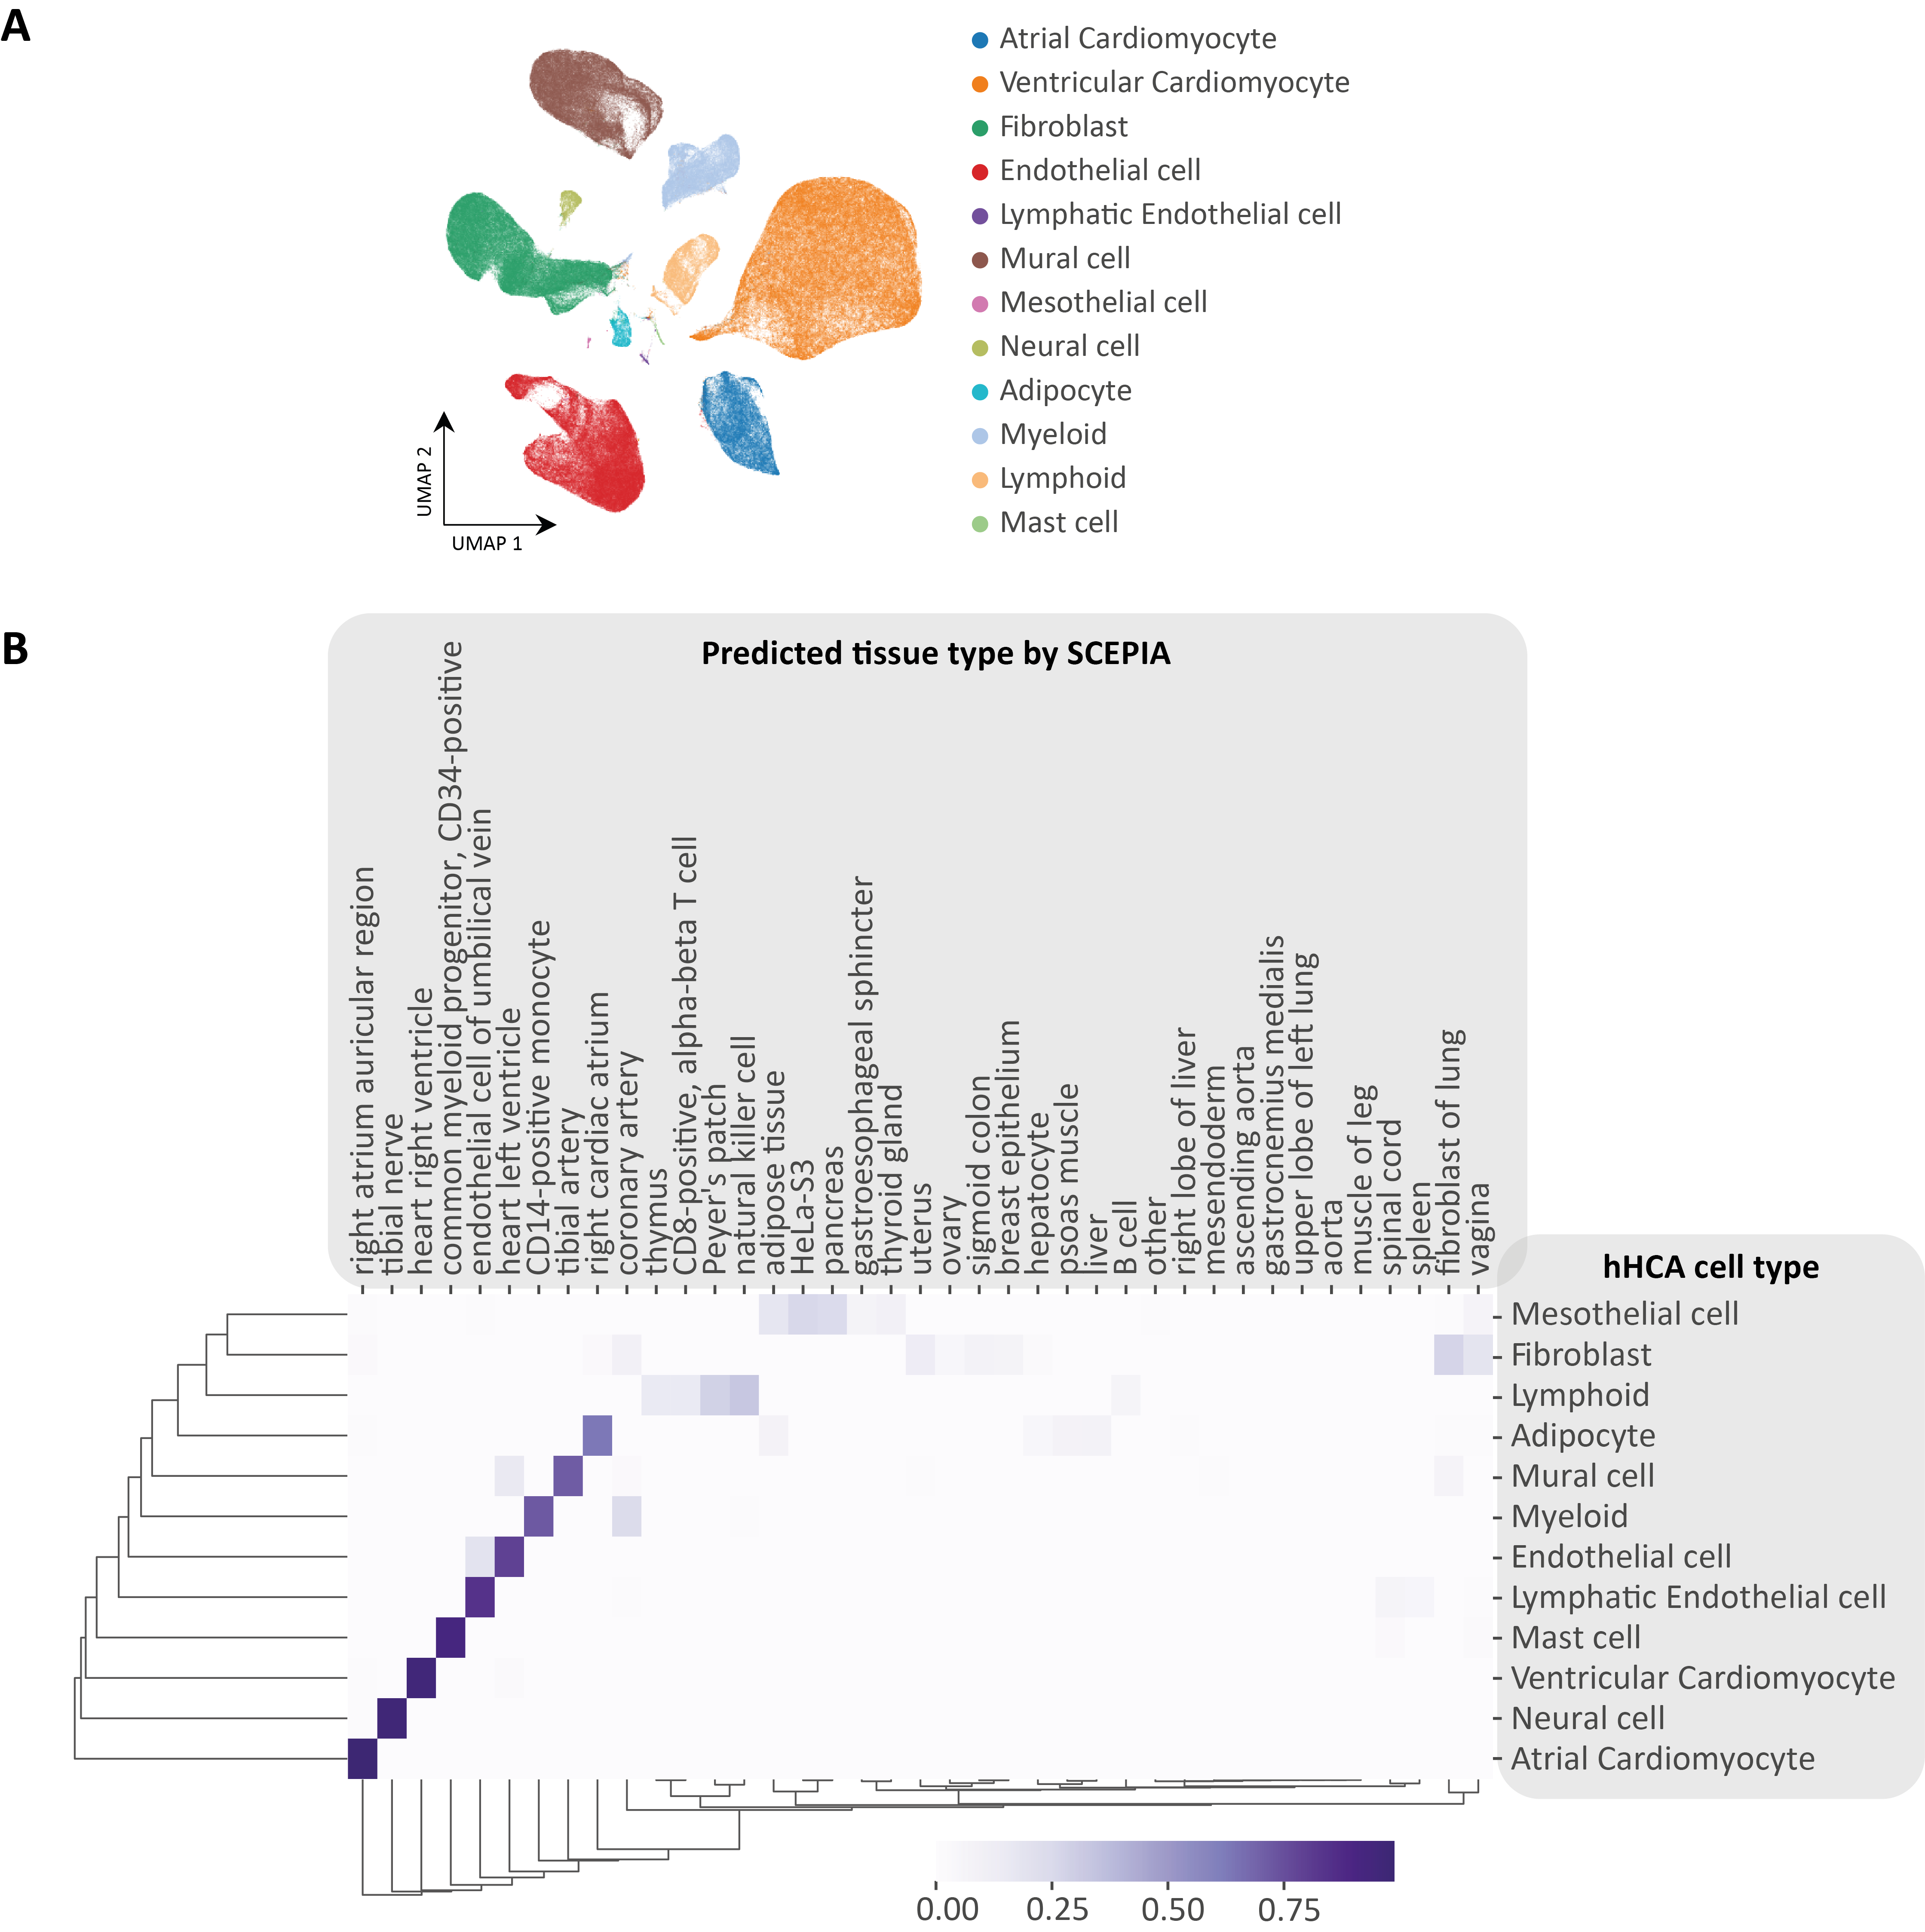
\includegraphics[width=\linewidth]{ch.scepia/imgs/SCEPIA_Annotation_allCells_SuppFig1_v4.png}
    \caption{Original annotation of cell types (a) SCEPIA annotation of clusters (b) Highest scoring motifs inferred with SCEPIA run on 700K cells (placeholder) }
    \label{fig:scepia_annotation1}
\end{figure}

\begin{figure}
    \centering
    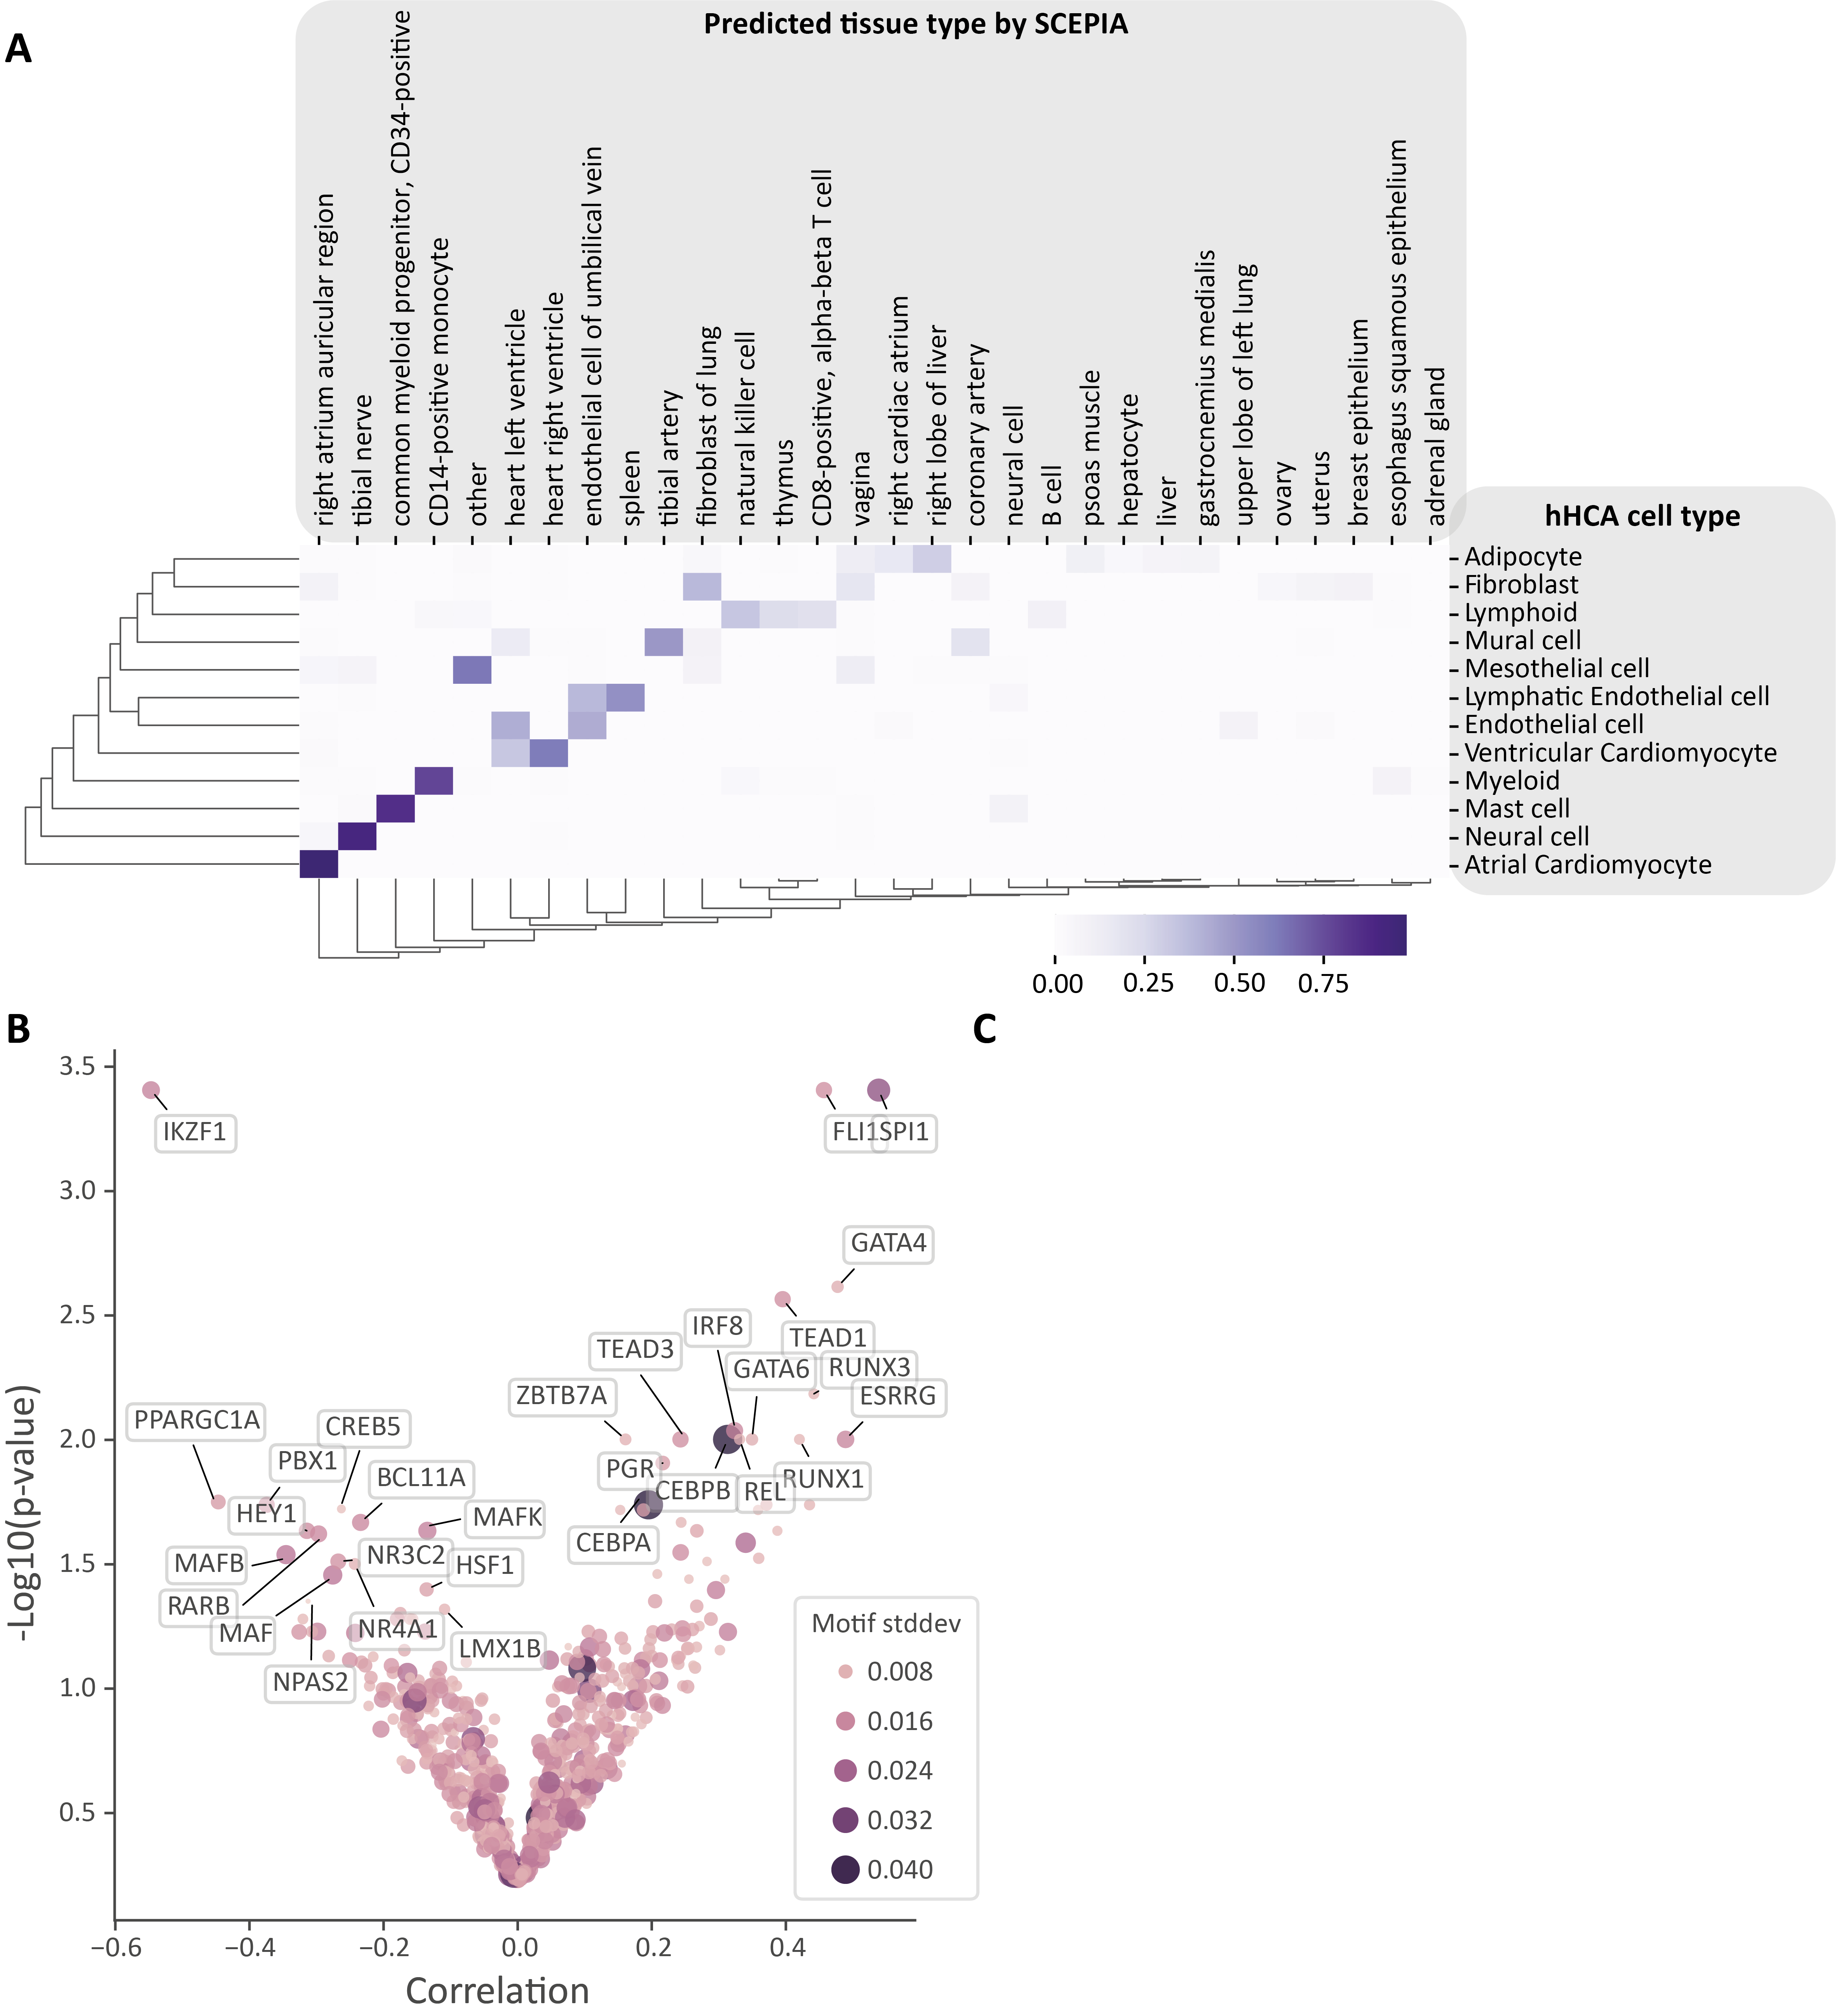
\includegraphics[width=\linewidth]{ch.scepia/imgs/SCEPIAGEOSKETCH_AllCells20000_Suppfig_v2.png}
    \caption{SCEPIA run on geosketch of hHCA (A) SCEPIA annotation of clusters (B) Highest scoring motifs inferred with SCEPIA run on 700K cells (C) (placeholder XX) UMAP of 20K geosketch hHCA. }
    \label{fig:geoscepia_results}
\end{figure}

\begin{figure}
    \centering
    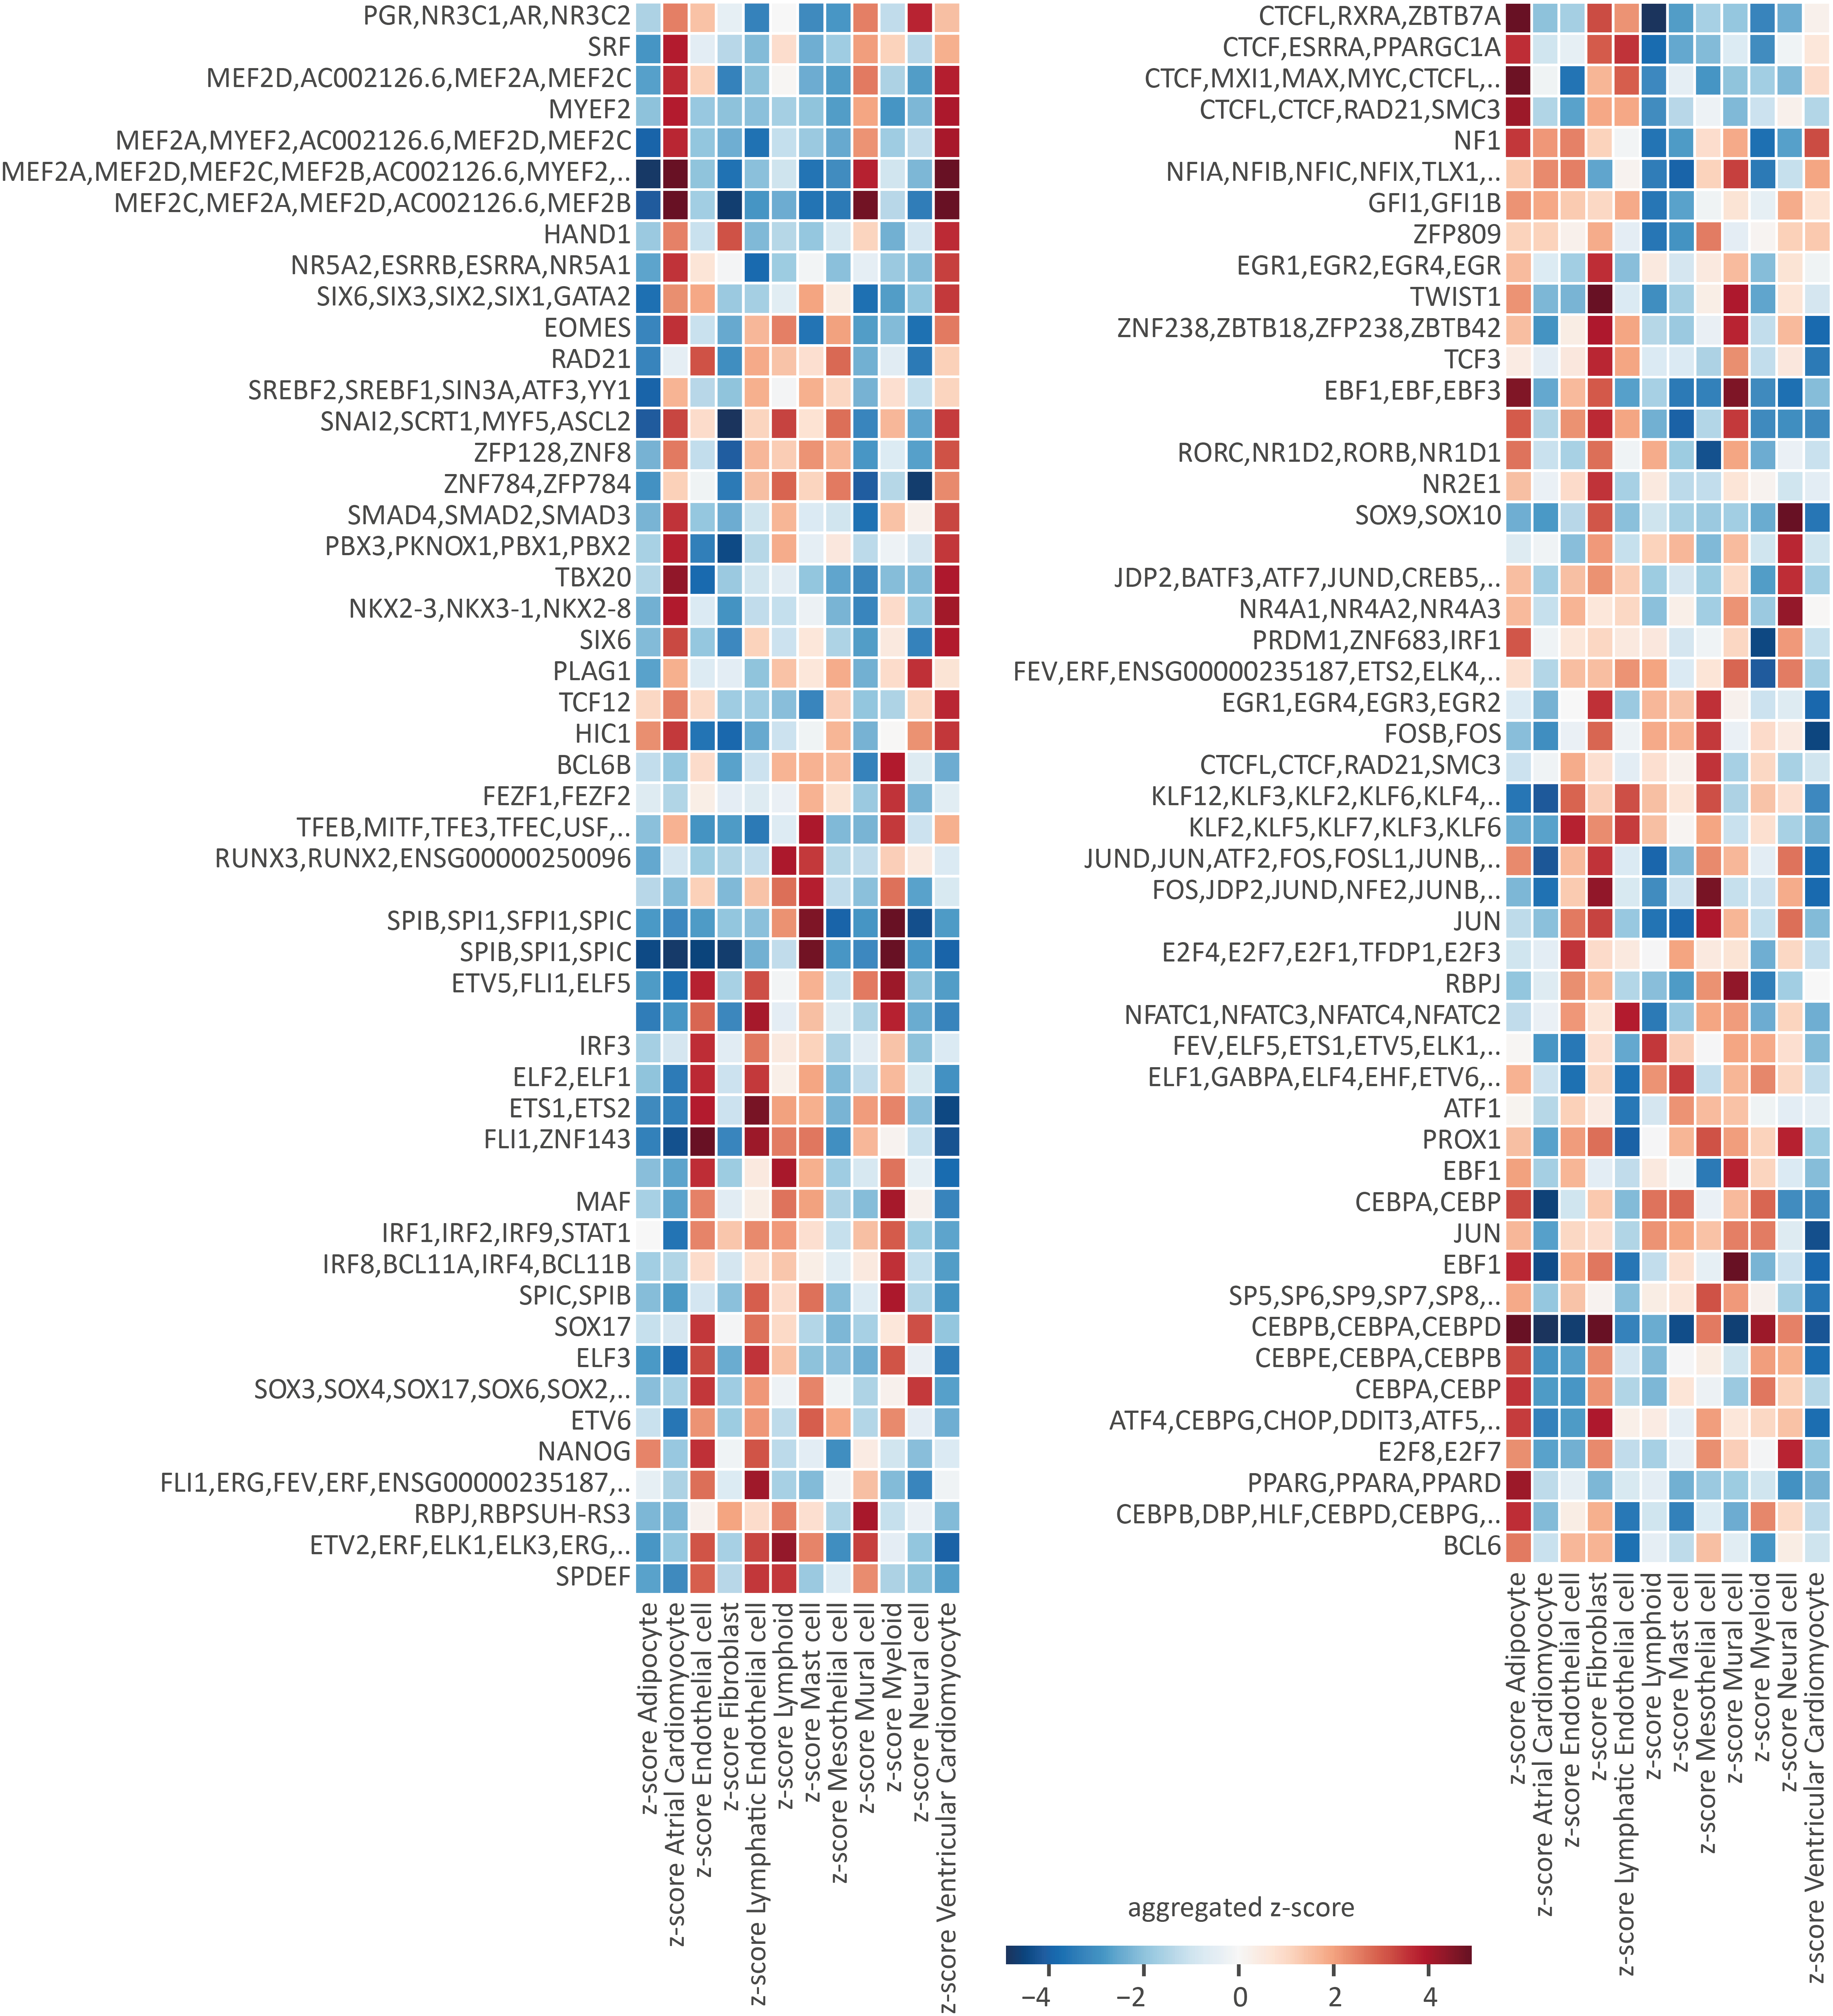
\includegraphics[width=\linewidth]{ch.scepia/imgs/Maelstrom_AllHitsAbove3.5.png}
    \caption{Maelstrom motif analysis output (z-score > 3.5) of the hHCA scATAC-seq cluster averages.}
    \label{fig:scepia_maelstromhm}
\end{figure}
\begin{figure}
    \centering
    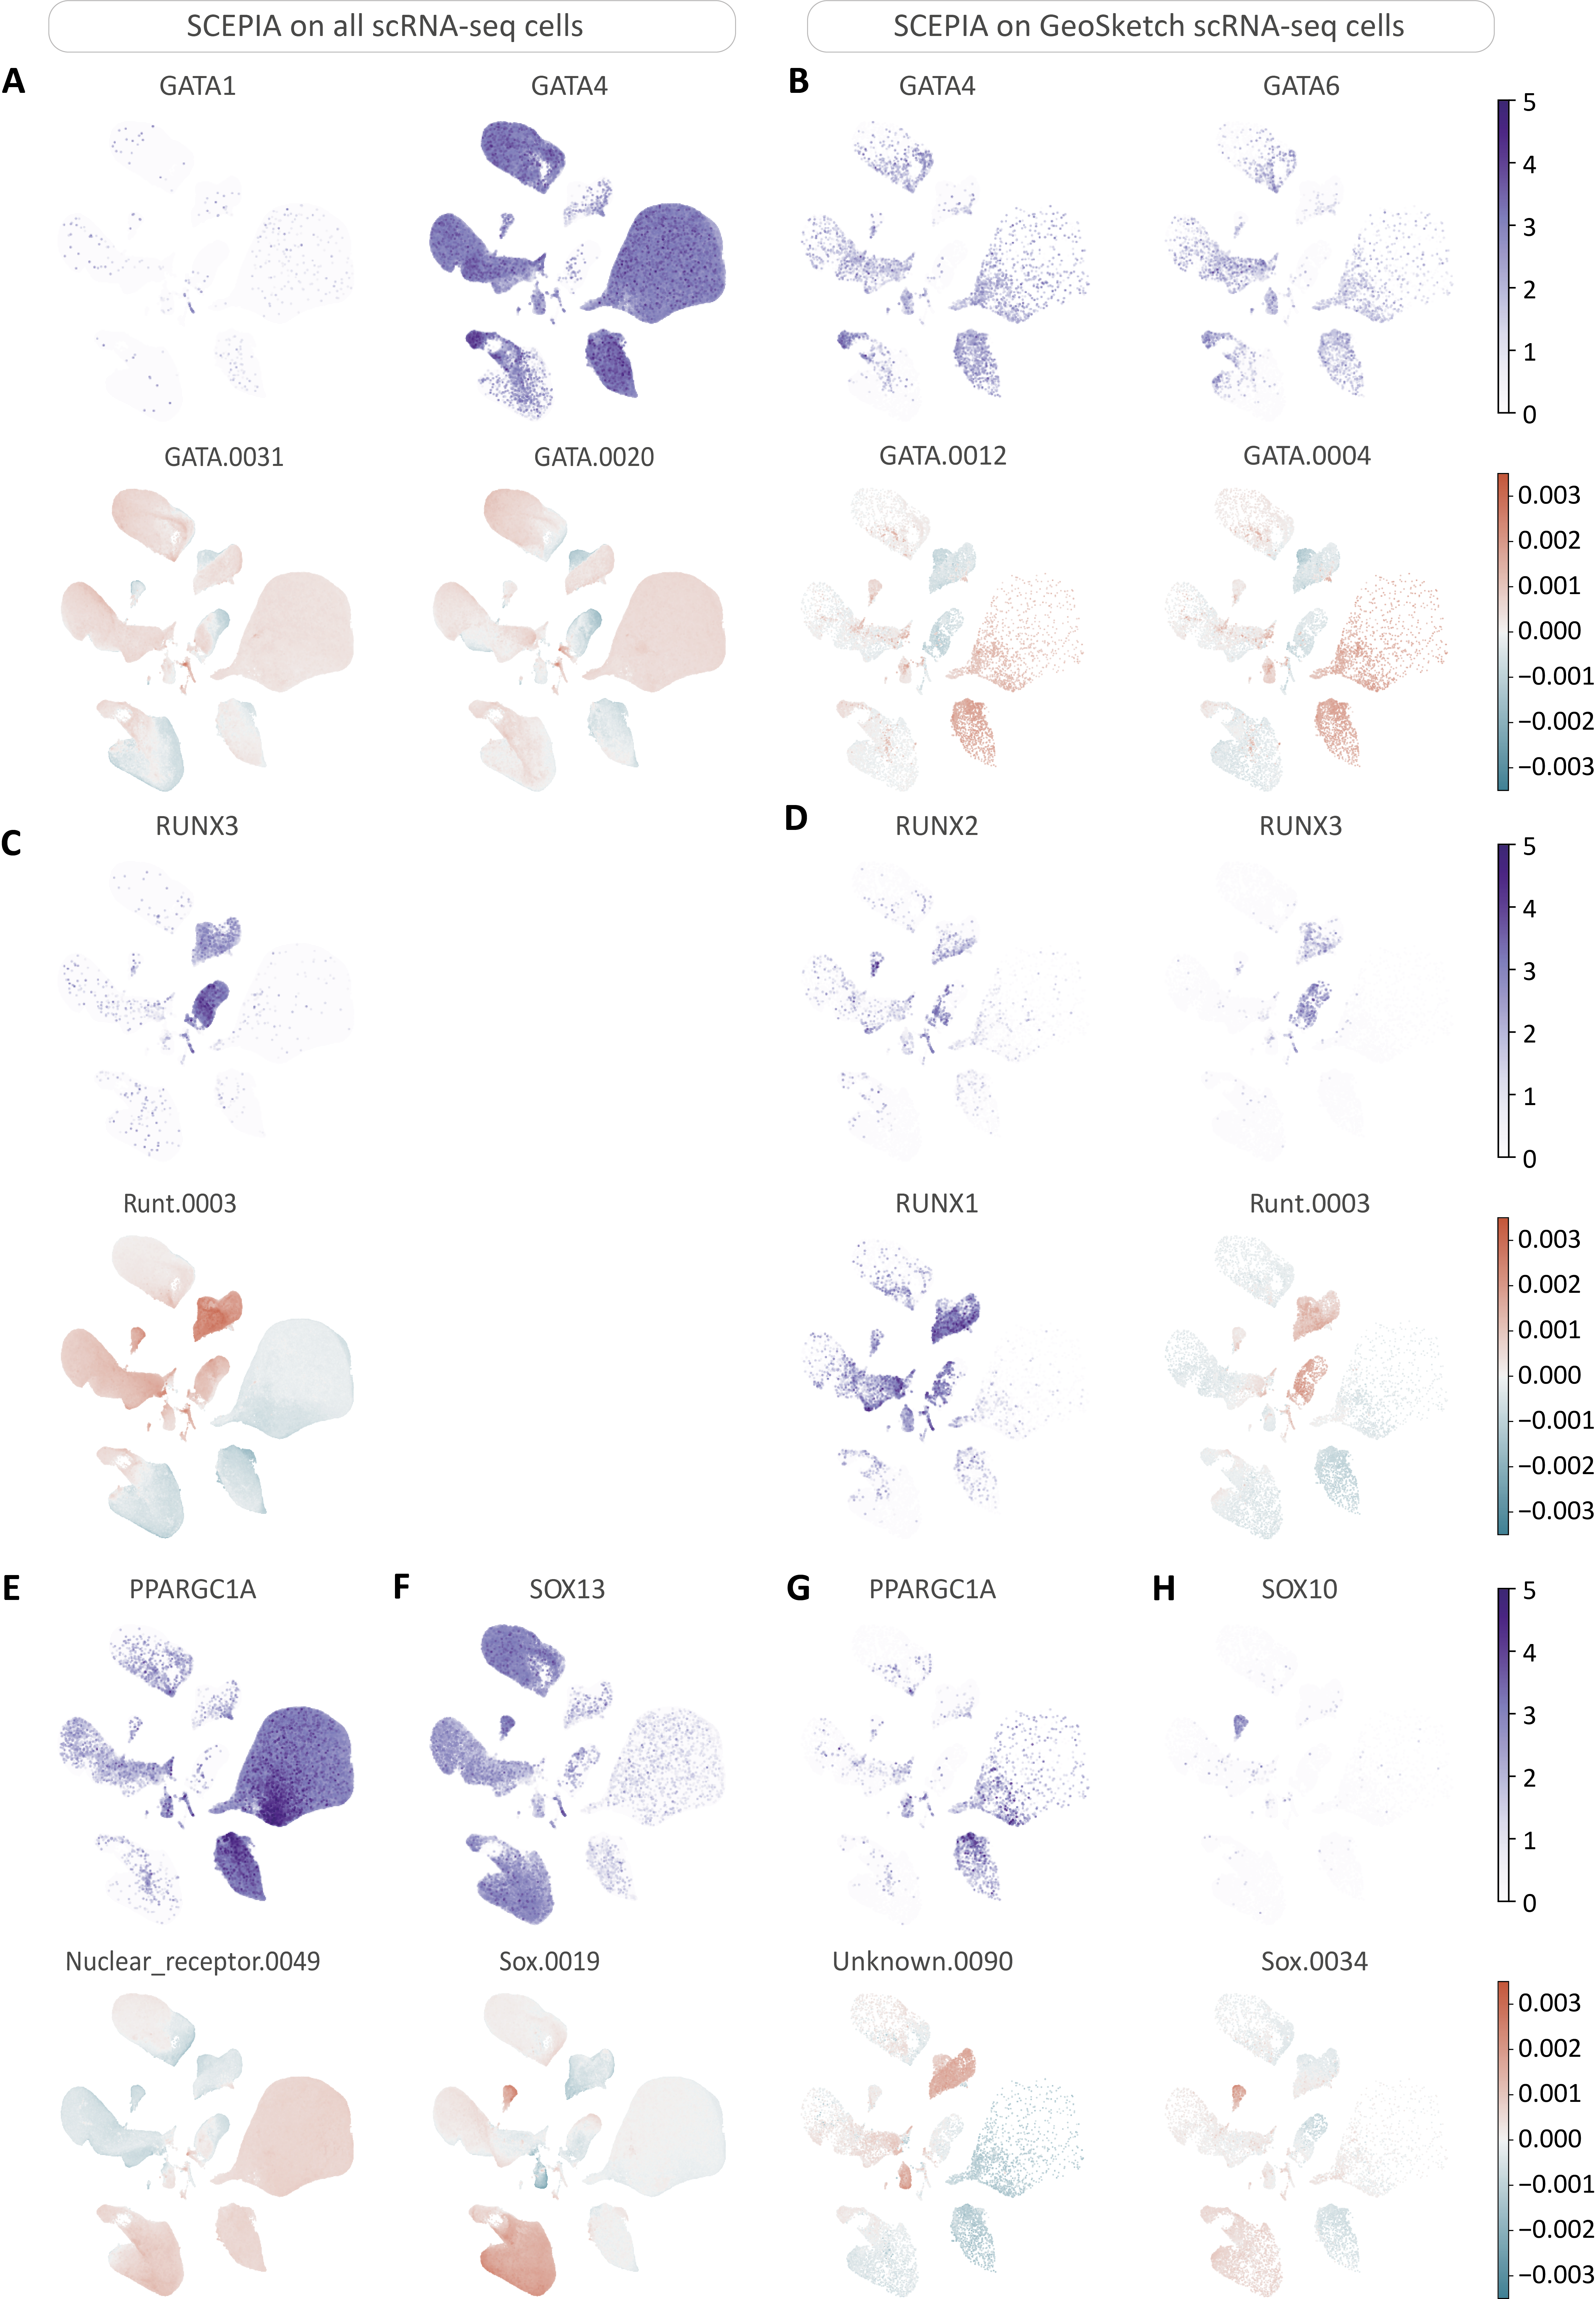
\includegraphics[width=\linewidth]{ch.scepia/imgs/SCEPIA_SCEPIAGEO_BiologicalExamples_SuppFig1_v2.png}
    \caption{Examples of SCEPIA and geosketch + SCEPiA run}
    \label{fig:scepia_features1}
\end{figure}

\begin{figure}
    \centering
    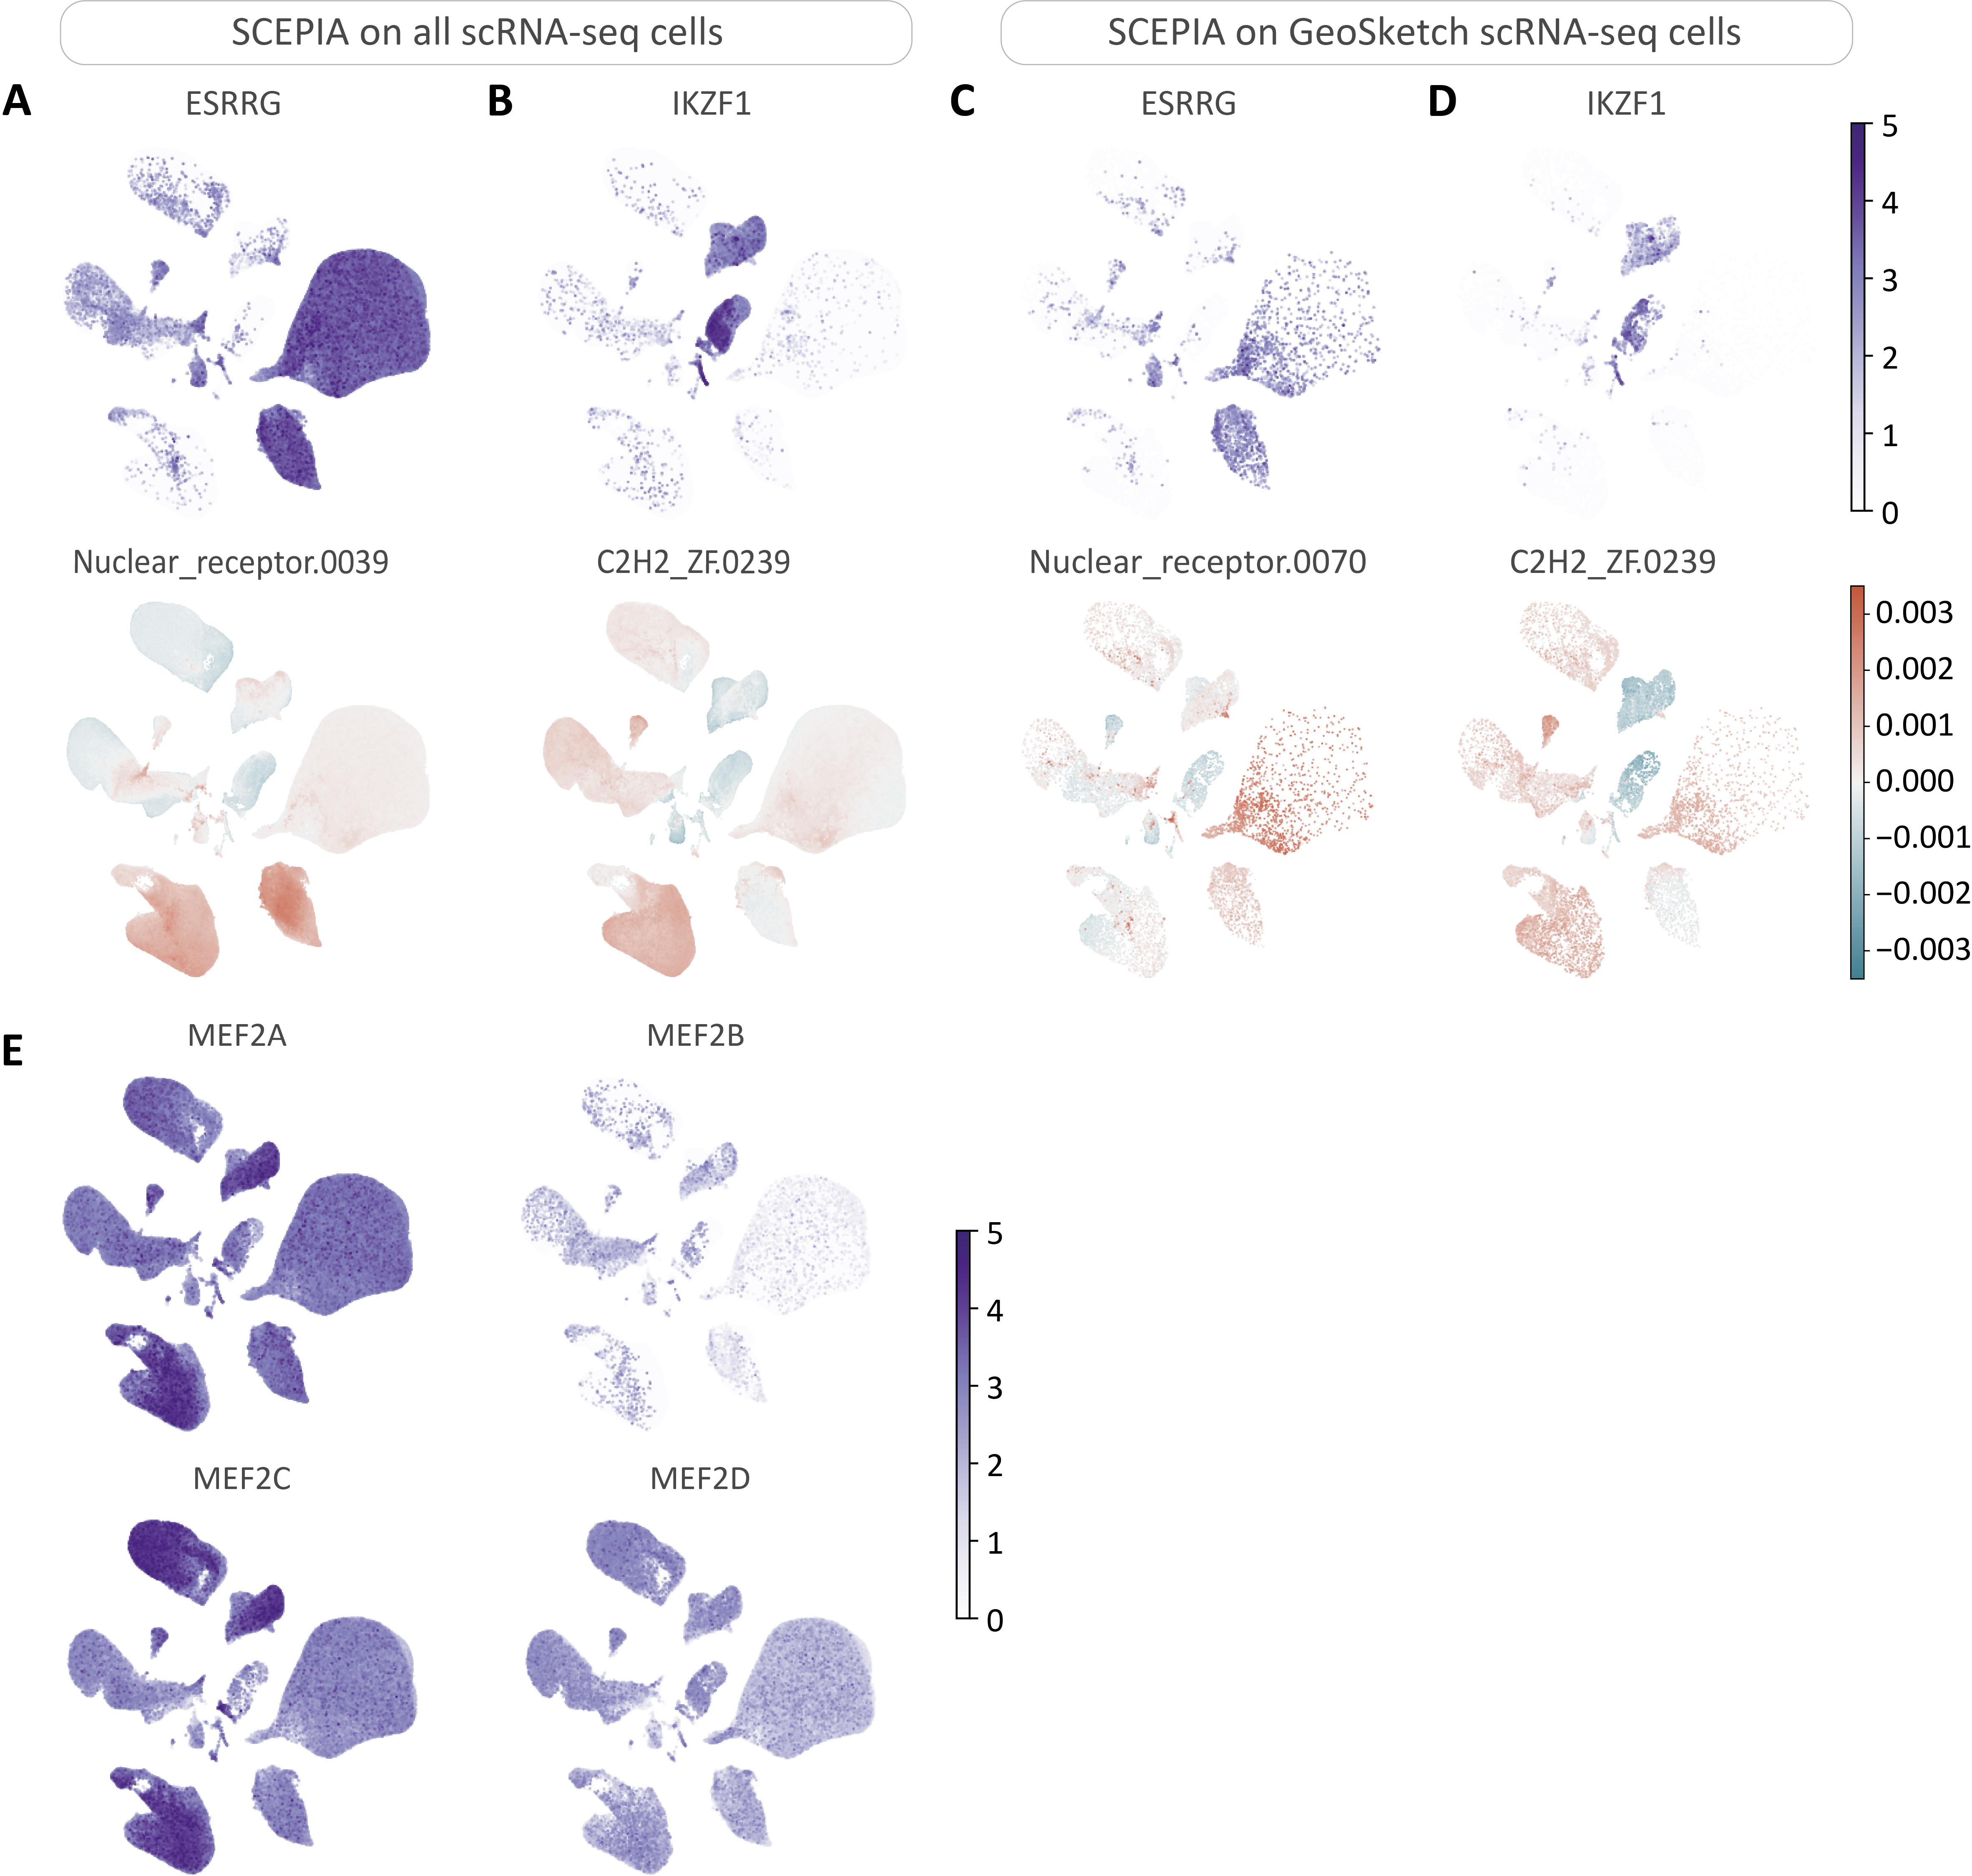
\includegraphics[width=\linewidth]{ch.scepia/imgs/SCEPIA_SCEPIAGEO_BiologicalExamples_SuppFig2_v2.png}
    \caption{Examples of SCEPIA and geosketch + SCEPiA run}
    \label{fig:scepia_features2}
\end{figure}